\PassOptionsToPackage{dvipsnames,svgnames,table}{xcolor}
\documentclass[11pt]{article}
\usepackage[a4paper,margin=22mm]{geometry}
\usepackage[no-math]{fontspec}
\setmainfont{DejaVu Serif}
\usepackage{amsmath,amssymb,amsthm,mathtools,graphicx,xcolor,hyperref,xurl,xspace,ifthen,enumerate}
\usepackage[shortlabels]{enumitem}
\setlength{\emergencystretch}{4em}
\AtBeginDocument{\special{pdf:mapline pzdr Dingbats <uzdr.pfb}}
\SetMathAlphabet{\mathbf}{normal}{OT1}{cmr}{bx}{n}
\SetMathAlphabet{\mathbf}{bold}{OT1}{cmr}{bx}{n}
\newtheorem{theo}{Theorem}[section]
\newtheorem{lemm}[theo]{Lemma}
\newtheorem{thm}[theo]{Theorem}
\newtheorem{proposition}[theo]{Proposition}
\newtheorem{corollary}[theo]{Corollary}
\newtheorem{definition}[theo]{Definition}
\newtheorem{theorem}[theo]{Theorem}
\newtheorem*{remas*}{Remarks}
\newtheorem{remas}[theo]{Remarks}
\newtheorem*{exam*}{Example}
\newtheorem{ques}[theo]{Question}
\providecommand{\og}{«\nobreakspace}
\providecommand{\fg}{\nobreakspace»}
\newtheorem{lem}[theo]{Lemma}
\newtheorem{lemma}[theo]{Lemma}
\newtheorem{prop}[theo]{Proposition}
\newtheorem{coro}[theo]{Corollary}
\newtheorem{corol}[theo]{Corollary}
\newtheorem*{conj*}{Conjecture}
\newtheorem{conj}[theo]{Conjecture}
\newtheorem{conjecture}[theo]{Conjecture}
\newtheorem{Proposition}[theo]{Proposition}
\newtheorem{theoreme}[theo]{Theorem}
\theoremstyle{definition}
\newtheorem{defi}[theo]{Definition}
\newtheorem{exam}[theo]{Example}
\newtheorem{exem}[theo]{Example}
\newtheorem{remark}[theo]{Remark}
\newtheorem{example}[theo]{Example}
\newtheorem{exams}[theo]{Examples}
\newtheorem{rema}[theo]{Remark}
\newtheorem{nota}[theo]{Notation}
\newtheorem{notation}[theo]{Notation}
\newtheorem*{notas}{Notations}
\newtheorem{result}[theo]{Result}
\newtheorem{question}[theo]{Question}
\newtheorem{prob}[theo]{Problem}
\newtheorem*{rema*}{Remark}
\newtheorem*{defi*}{Definition}
\newtheorem*{theo*}{Theorem}
\newtheorem*{lemm*}{Lemma}
\newtheorem*{prop*}{Proposition}
\newcommand{\enoncename}{}
\newtheorem{corpusenonce}[theo]{\enoncename}
\newenvironment{enonce}[2][]{\renewcommand{\enoncename}{#2}\begin{corpusenonce}}{\end{corpusenonce}}
\newenvironment{enonce*}[2][]{\par\medskip\noindent\textbf{#2.}\itshape}{\par\medskip}
\newenvironment{proofc}[1][\proofname]{\begin{proof}[#1]}{\end{proof}}
\newcommand{\Mc}{\mathcal{M}}
\newcommand{\pointir}{.\ ---\ }
\newcommand{\equalenv}[2]{\expandafter\let\csname#1\expandafter\endcsname\csname#2\endcsname\expandafter\let\csname end#1\expandafter\endcsname\csname end#2\endcsname}
\providecommand{\diagbox}[3][]{\begin{tikzpicture}[x=1em,y=1em,baseline=(current bounding box.center)]\useasboundingbox(0,0) rectangle(3,1.4);\draw(0,1.4)--(3,0);\node at(.5,.3){#2};\node at(2.5,1.1){#3};\end{tikzpicture}}
\providecommand{\eg}{e.g.\ }
\providecommand{\ie}{i.e.\ }
\providecommand{\cf}{cf.\ }
\providecommand{\longthanks}[1]{\par\smallskip\noindent #1\par\smallskip}
\providecommand{\qbinom}[2]{\genfrac{[}{]}{0pt}{}{#1}{#2}}

\providecommand{\mathof}[1]{\mathrm{#1}}

\numberwithin{equation}{section}


\def\endappendix{}


\usepackage{multirow,tikz, blkarray, mathrsfs,scalerel,stackengine}
\usetikzlibrary{arrows,matrix,positioning}

\stackMath
\newcommand\reallywidehat[1]{\savestack{\tmpbox}{\stretchto{\scaleto{ \scalerel*[\widthof{\ensuremath{#1}}]{\kern.1pt\mathchar"0362\kern.1pt}{\rule{0ex}{\textheight}}}{\textheight}}{2.4ex}}\stackon[-6.9pt]{#1}{\tmpbox}}

\newcommand{\N}{\mathbb{N}}
\newcommand{\C}{\mathbb{C}}
\newcommand{\Q}{\mathbb{Q}}
\newcommand{\Z}{\mathbb{Z}}
\newcommand{\R}{\mathbb{R}}
\newcommand{\K}{\mathbb{K}}
\newcommand{\F}{\mathbb{F}}
\newcommand{\Lq}{\mathbb{K}}
\newcommand{\ZZ}{\widetilde{Z}}

\newcommand{\Kostka}{K_{\lambda \mu}}
\newcommand{\Stab}{\operatorname{Stab}}
\newcommand{\Spann}{\text{-}\operatorname{span}}
\DeclareMathOperator{\Sym}{Sym}
\DeclareMathOperator{\aff}{aff}
\newcommand{\en}{e^+_{[1,n-k]}}
\newcommand{\enn}{e^+_{[1,n-k-1]}}
\newcommand{\ep}{e^+}
\newcommand{\eplusB}{e^+_{[k+1,n]}}
\newcommand{\Sn}{S_{[1,n-k]}}
\newcommand{\Snn}{S_{[1,n-k-1]}}
\newcommand{\Snnn}{S_{[1,n-k+1]}}
\newcommand{\Stabn}{(S_{[1,n-k]})_\lambda}
\newcommand{\Stabnn}{\Stab_{[1,n-k-1]}}
\newcommand{\Stabnnn}{\Stab_{[1,n-k+1]}}
\newcommand{\Waff}{W_{\aff}}
\newcommand{\Wlambda}{\frac{1}{W^{n-k}_{\lambda}(t)}}
\newcommand{\Symm}[1]{\sum\limits_{w\in \Sn} T_w \left( #1 \right)}
\newcommand{\wmin}{w_{\lambda^-}}
\newcommand{\shatproduct}{s_1 \dotsm \widehat{s}_{t_1} \dotsm \widehat{s}_{t_r} \dotsm s_k}
\newcommand{\reversesproduct}{s_k \dotsm \widehat{s}_{t_r} \dotsm \widehat{s}_{t_1} \dotsm s_1}
\newcommand{\nusum}{\sum_{\nu\in S_{[k+1,n]}(\lambda)}}



\newcommand{\Mpoln}{\mathcal{M}_n^{pol}}
\newcommand{\Mpolnn}{\mathcal{M}_{n-1}^{pol}}



\newcommand{\Emu}{E_{(\mu \mid \gamma)}}
\newcommand{\Elambda}{E_{(\lambda \mid \gamma)}}
\newcommand{\EB}[1]{E_{#1}^\dagger}
\newcommand{\EBlong}[1]{E_{#1}^\dagger(z;q^{-1},t^{-1})}
\newcommand{\EI}[1]{E_{#1}}
\newcommand{\EIlong}[1]{E_{#1}(x;q,t)}
\newcommand{\E}[1]{E_{#1}}
\newcommand{\Estar}[1]{E^*_{#1}}
\newcommand{\Estarlong}[1]{E^*_{#1}(z;q,t)}
\newcommand{\PB}[1]{P_{#1}^\dagger}
\newcommand{\PBlong}[1]{P_{#1}^\dagger(z;q^{-1},t^{-1})}
\newcommand{\PP}{P_{(\lambda \mid \gamma)}}
\newcommand{\PPmin}{P_{(\lambda^- \mid \gamma)}}
\newcommand{\Pn}{P_{(\lambda \mid \gamma)}}
\newcommand{\Pnn}{P^{n-1}_{\gamma \mid \mu}(q,t)}
\newcommand{\Pinf}{P_{\gamma \mid \mu}(q,t)}
\newcommand{\JJ}{\mathcal{J}_{(\lambda \mid \gamma)}}
\newcommand{\MM}{\mathbb{M}_{\gammalambdamin}}
\newcommand{\MMM}{\mathbb{M}_{\lambdagamma}}
\newcommand{\CC}{\mathcal{A}^\lambdagamma_\mueta}


\newcommand{\numu}{{(\nu \mid \mu)}}
\newcommand{\munu}{{(\mu \mid \nu)}}
\newcommand{\numin}{{\nu^-}}
\newcommand{\nudom}{{( \lambda \mid \gamma )}}
\newcommand{\lambdagamma}{{\nudom}}
\newcommand{\gammalambdamin}{{(\gamma \mid \lambda^-)}}
\newcommand{\gammanu}{{(\gamma \mid \nu)}}
\newcommand{\nuantidom}{{(\lambda^- \mid \gamma)}}
\newcommand{\lambdak}{\lambda^{(n-k)}}
\newcommand{\numuprime}{{(\nu \mid \mu')}}
\newcommand{\etamu}{{(\eta \mid \mu^-)}}
\newcommand{\mueta}{{(\mu \mid \eta)}}
\newcommand{\etamuprime}{{(\eta \mid \mu')}}
\newcommand{\mutilde}{{\widetilde{\mu}}}
\newcommand{\lambdatilde}{{\widetilde{\lambda}}}
\newcommand{\gammalambdatilde}{{(\gamma \mid \lambdatilde)}}
\newcommand{\lambdatildegamma}{{(\lambdatilde \mid \gamma)}}
\newcommand{\lambdamingamma}{(\lambda^- \mid \gamma)}
\newcommand{\mumineta}{(\mu^- \mid \eta)}
\newcommand{\flambdatilde}{f_{\lambdatilde , \lambdagamma}}
\newcommand{\etamutilde}{{(\eta \mid \widetilde{\mu})}}
\newcommand{\nugamma}{{(\nu \mid \gamma)}}
\newcommand{\mugamma}{{(\mu \mid \gamma)}}
\newcommand{\mutildeeta}{{(\mutilde \mid \eta)}}
\newcommand{\etamumin}{{(\eta \mid \mu^-)}}
\newcommand{\fmuu}{f_{\mu, \lambdagamma}}


\newcommand{\chin}{q^{\ell_\mu(u)+1}t^{a_\mu(u)}}
\newcommand{\jj}{j_{(\lambda \mid \gamma)}}
\newcommand{\pIone}{p_{I_1}(\overline{z})}
\newcommand{\tildepIone}{\widetilde{p}_{I_1}}
\newcommand{\pIoneevaluated}{p_{I_1}\left(\overline{\etamutilde}\right)}
\newcommand{\pItwo}{p_{2}(\overline{z})}
\newcommand{\pItwoevaluated}{p_{2}\left(\overline{\etamutilde}\right)}
\newcommand{\mIone}{m_{\etamu}^{\gammalambdamin}}
\newcommand{\mIoneprime}{m_{\mueta}^{\lambdagamma}}
\newcommand{\hIone}{h}
\newcommand{\dI}{d_I}
\newcommand{\fnu}{f_{\nu, \gammalambdamin}}
\newcommand{\fnuu}{f_{\nu,\lambdagamma}}
\newcommand{\fmu}{f_{\mu,\lambdagamma}}
\newcommand{\fsimu}{{f_{s_i(\mu),\lambdagamma}}}
\newcommand{\gmutilde}{f_{\mutilde,\etamu}}
\newcommand{\fmutilde}{f_{\mutilde, \mueta}}
\newcommand{\gmuprime}{f_{\mu',\etamu}}
\newcommand{\betaa}{{q^{\ell_{s_i(\mu)}(u)+1} t^{a_{s_i(\mu)}(u)}}}



\newcommand{\leg}[1]{{\ell_{#1}(\square)}}
\newcommand{\legnu}{{\ell_\nu(\square)}}
\newcommand{\legnumin}{{\ell_{\nu^-}(\square)}}
\newcommand{\armone}[1]{{\widetilde{a}_{#1}(\square)}}
\newcommand{\armonenu}{{\widetilde{a}_\nu(\square)}}
\newcommand{\armonenumin}{{\widetilde{a}_{\nu^-}(\square)}}
\newcommand{\armtwo}[1]{{a_{#1}(\square)}}
\newcommand{\armtwonu}{{a_\nu(\square)}}
\newcommand{\armtwonumin}{{a_{\nu^-}(\square)}}
\newcommand{\armdelta}{{a_\delta(\square)}}
\newcommand{\coarm}{{a'_\mu(\square)}}
\newcommand{\symmetricprod}{\prod\limits_{\square \in \lambda^-}}
\newcommand{\nonsymmetricprod}{\prod\limits_{\square \in \gamma}}

\newcommand{\group}[1]{\operatorname{Group}\,\operatorname{#1}}

\newcommand{\jone}{j_1}
\newcommand{\jtwo}{j_2}
\newcommand{\jthree}{j_3}
\newcommand{\jfour}{j_4}
\newcommand{\jfive}{j_5}
\newcommand{\Estarone}{E^*_1}
\newcommand{\Estartwo}{E^*_2}
\newcommand{\Estarthree}{E^*_3}
\newcommand{\Estarfour}{E^*_4}
\newcommand{\Estarfive}{E^*_5}
\newcommand{\ltm}{\ell'_{t_u}}
\newcommand{\lj}{\ell'_j}
\newcommand{\lh}{\ell'_h}

\newcommand{\RS}{\mathrm{R_{S}}(x)}
\newcommand{\RNS}{\mathrm{R_{NS}}(x)}
\newcommand{\LL}{\mathrm{LL}(x)}
\newcommand{\RL}{\mathrm{RL}(x)}
\newcommand{\cbox}{c(\square)}

\newcommand{\DBaratta}{D_{\etamumin}^\gammalambdamin}
\newcommand{\DHHL}{D_{\mueta}^\lambdagamma}
\newcommand{\dtwo}{d'_I}
\newcommand{\nutilde}{\widetilde{\nu}}
\newcommand{\gammanutilde}{{(\gamma \mid \nutilde)}}
\newcommand{\pstarone}{p^*_{I'_1}}
\newcommand{\pstartwo}{p^*_2}
\newcommand{\pstarthree}{p^*_{I'_3}}

\newcommand{\Inv}{\mathrm{Inv}}

\newcommand{\Aqt}{\mathbb{A}_{q,t}}
\newcommand{\Atq}{\mathbb{A}_{t,q}}
\newcommand{\At}{\mathbb{A}_t}
\newcommand{\id}{\mathsf{e}}

\newcommand{\PFH}{\mathrm{PFH}}

\newcommand{\Hilb}{\mathrm{Hilb}}

\newcommand{\Hom}{\mathrm{Hom}}

\newcommand{\T}{\mathbb{T}}

\newcommand{\wt}{\mathrm{wt}}

\newcommand{\Y}{\mathbb{Y}}
\newcommand{\dg}{d}
\newcommand{\dga}{\widehat{\dg}}
\newcommand{\tT}{\tilde{T}}
\newcommand{\fixit}[1]{{\tt \color{blue} *** #1 ***}}

\allowdisplaybreaks




\date{July 1, 2024}










\begin{document}
\section*{\raggedright 1005: Degree-one symmetric-block Pieri formula for type-A partially symmetric Macdonald polynomials}
\noindent\textbf{Author:} Goodberry, Ben\par\noindent\textbf{Source:} Type A partially-symmetric Macdonald polynomials. Algebraic Combinatorics 7 (2024), publisher version, DOI 10.5802/alco.388. \url{https://alco.centre-mersenne.org/articles/10.5802/alco.388/}
\par\noindent\textbf{License:} CC BY 4.0, \url{https://creativecommons.org/licenses/by/4.0/}. The original publisher PDF cover has the explicit license notice. See the saved source/license records.
\par\noindent\textbf{Editorial material note (not author text):} The selected problem is original Theorem4.9 only, the degree-one symmetric-block Pieri expansion for the exact type-A partially-symmetric Macdonald polynomials and stated support/coefficient conventions. Complete author Sections1--4 retain normalization, Hecke/interpolation identities, unique maximal-index support construction and every coefficient evaluation/ratio calculation901--963; full local decreasing-T and nonvanishing proofs are retained in author Appendices2103--2138. The later nonsymmetric-variable formula and coefficient-cancellation/simplification program are unselected context/applications, not extra units. All diagrams are editable author TikZ and the exact original reallywidehat macro resolves through installed genuine scalerel/stackengine, without accent/font substitutions. Every proof paragraph and formula remains native human-authored TeX, with no assistant-generated proof or mathematical repair. All proof text and formulas below are editable author TeX. Mathematical wording, language and proof order are retained. Only the article class, title matter and bibliography presentation are adapted for independent compilation; no proof has been generated or repaired.
\par\noindent\textbf{Editorial difficulty:} H3: The proof derives a unique admissible support parametrization by Hecke-operator expansions, reverses interpolation-Macdonald evaluations and solves the coefficient ratios at every support point. Full maximal-index choice, normalization and denominator/evaluation formulas are preserved, beyond a formal specialization of a symmetric Pieri rule.
\medskip\hrule\medskip
\noindent\textbf{Author statement, complete proof and local supporting text follow in source order.}
\section{Introduction}
The type $GL_n$ nonsymmetric Macdonald polynomials can be symmetrized, for example by acting on $E_\mu$ by a symmetrization operator over the finite Weyl group, to obtain the classic symmetric Macdonald polynomials. In recent work~\cite{Schlosser}, Schl\"{o}sser constructs a symmetrization over a parabolic subgroup $W_J$ for nonsymmetric Macdonald polynomials in general type. This was done in type $GL_n$ by Lapointe~\cite{Lapointe} for a particular choice of parabolic subgroup, with the goal of building a basis for partially-symmetric polynomials which are Schur-positive for some $m$-symmetric form of Schur polynomials. We will use the same type of construction, with the symmetric group $S_{[1,n-k]}$ acting on the first $n-k$ variables as our parabolic subgroup, which gives us polynomials that are stable when adding symmetrized variables. This stability is special to type $A$, and to this parabolic subgroup.

In order to build an integral form $\JJ$ as a normalization of $\PP$, in Section~\ref{diagrams} we introduce Young diagram statistics associated with the split diagram $\lambdagamma$. This includes a different way to count arms depending on whether the column is in the symmetric part of the diagram $\lambda$, or the nonsymmetric part $\gamma$. These coincide with the integral form of the $m$-symmetric Macdonald polynomials in~\cite{Lapointe}. We use the combinatorial formula for the nonsymmetric Macdonald polynomials found in~\cite{MR2405160} in order to prove that $\JJ \in \mathbb{Z}[q,t][x_1, \dotsc, x_n]$ in Section~\ref{integralformsection}. This is mentioned but not proven in~\cite{Lapointe}.

The major new identities we explore that do not seem to appear elsewhere are rules for multiplication of $\PP$ by either $e_1[x_1, \dotsc, x_{n-k}]$, the elementary symmetric polynomial in all of the symmetrized variables, or by $x_j$ where $j>n-k$, a nonsymmetric variable. We derive these formulas in Section~\ref{ElementaryMultiplication}. Our approach for finding formulas for these products, written in the basis of partially-symmetric Macdonald polynomials, uses a similar approach by Baratta in~\cite{MR2525842} for the product $x_i E_\mu$. Namely, this makes heavy use of the interpolation nonsymmetric Macdonald polynomials of Knop~\cite{MR1456318} and Sahi~\cite{MR1399411}. Halverson and Ram~\cite{MR4756478} find Monk type formulas for the same products, but instead using Cherednik's intertwiners. While these formulas could be symmetrized in a naive way, combining the resulting expansion to get it into the basis of partially-symmetric Macdonald polynomials is quite difficult, as many terms combine to the same $P_{\mueta}$. We get around this using properties of the Hecke operators and by evaluating the interpolation polynomial expressions at a special point which forces uniqueness and avoids any overlapping of terms.

Our primary goal is to build the polynomials which appear in~\cite{MR4081116} as isomorphic images of fixed points of a torus action in the Parabolic Flag Hilbert scheme, which will be established in upcoming works with D. Orr and M. Bechtloff Weising. Toward this end, after finding a formula for the expansion of $e_1[x_1, \dotsc, x_{n-k}] \PP$, in Section~5 we categorize many combinatorial simplifications that can be made to that formula.

This article includes the majority of the results submitted for a doctoral dissertation in~\cite{Dissertation}, though the final simplifications and $x_j \PP$ formulas do not appear there.



\section{Partially symmetric Macdonald polynomials}

\subsection{Nonsymmetric Macdonald polynomials}

Let $\K=\Q(q,t)$ and $n>0$. For any composition $\nu\in(\Z_{\ge 0})^n$, denote by $E_\nu =E_\nu(x;q,t)\in \K[x_1,\dotsc,x_n]$ the nonsymmetric Macdonald polynomial of type $GL_n$ as defined in ~\cite{MR2405160}. These satisfy the triangularity property,
\begin{equation}\label{Etriangularity} E_\mu \in x^\mu + \sum_{\nu <_{\text{(Bru)}} \mu} c_\nu x^\nu,\end{equation}
where $x^\mu = x_1^{\mu_1} \dotsm x_n^{\mu_n}$, each $c_\nu \in \K[x_1,\dotsc, x_n]$, and $<_{\text{(Bru)}}$ is the Bruhat order. The symmetric group $S_n$ acts naturally on $\Z^n$ and $\K[x_1,\dotsc,x_n]$. For $1\le i<n$, let $s_i$ be the simple transposition $(i,i+1)\in S_n$. Then explicitly, the Bruhat order is the partial ordering on compositions with the covering relations.
\begin{itemize}
    \item If $\mu_i > \mu_{i+1}$, then $s_i(\mu) > \mu$.
    \item If $\mu_{i+1}-\mu_i > 1$, then $s_i(\mu) > \mu + e_i - e_{i+1}$.
\end{itemize}
In this ordering, we consider a weakly-decreasing weight to be dominant, and a weakly-increasing weight antidominant.

Define the Demazure-Lusztig operators,
\begin{align*}
T_i = ts_i + \frac{(t-1)x_{i+1}}{x_{i+1}-x_i}(1-s_i), \qquad 1\le i<n.
\end{align*}
These satisfy the braid relations,
\begin{equation}\label{braidrelations}T_i T_{i+1} T_i = T_{i+1} T_i T_{i+1}, \qquad 1\leq i < n\end{equation}
\begin{equation} T_i T_j = T_j T_i \qquad \text{ if } |i-j|\geq 2\end{equation}
and the quadratic relations,
\begin{equation}\label{quadratic}
(T_i-t)(T_i+1)=0.
\end{equation}
For any reduced expression $w=s_{i_1}\dotsm s_{i_\ell}\in S_n$, we define the operator $T_w=T_{i_1}\dotsm T_{i_\ell}$. 

\subsection{Partially symmetric Macdonald polynomials}
Suppose $n>0$ and $k\geq 0$. We can regard $\Sn$ as the subgroup of $S_n$ fixing the elements $\{n-k+1,\dotsc,n\}$. Define the partial Hecke symmetrizer
$$
\en=\sum_{w\in \Sn} T_w.
$$
For $\lambda\in(\Z_{\ge 0})^{n-k}$, let $(\Sn)_\lambda\subseteq \Sn$ be its stabilizer and
\begin{align*}
W_\lambda(t)=\sum_{w\in (\Sn)_\lambda} t^{\ell(w)}.
\end{align*}


We write $\nu = (\lambda \mid \gamma)$ to indicate a splitting of a composition $\nu$ into two compositions, $\lambda$ and $\gamma$, i.e., $\nu=(\nu_1,\dotsc,\nu_n)=(\lambda_1,\dotsc,\lambda_{n-k},\gamma_1,\dotsc,\gamma_k)$ where $\lambda=(\lambda_1,\dotsc,\lambda_{n-k})\in(\Z_{\ge 0})^{n-k}$ and $\gamma=(\gamma_1,\dotsc,\gamma_k)\in(\Z_{\ge 0})^k$.

\begin{defi}
For a weakly-decreasing partition $\lambda \in (\mathbb{Z}_{\geq 0})^{n-k}$ and a composition $\gamma\in (\Z_{\ge 0})^k$, the partially symmetric Macdonald polynomial $P_{(\lambda|\gamma)}=P_{(\lambda|\gamma)}(x;q,t)$ is defined by
\[
P_{(\lambda|\gamma)} = \frac{\en  E_{(\lambda|\gamma)}}{W_\lambda(t)}.
\]
\end{defi}





\subsection{Diagrams and their statistics}\label{diagrams} In constructions related to compositions and their diagrams, we mostly follow the conventions of~\cite{MR2405160}. Compositions are tuples $\nu=(\nu_1,\dotsc,\nu_n)\in(\Z_{\ge 0})^n$. A composition $\nu$ is a partition if its entries are weakly decreasing. 

The diagram of a composition $\nu\in(\Z_{\ge 0})^n$ is the subset $\dg(\nu)\subset (\Z_{\ge 0})^2$ given by
$$ \dg(\nu)=\{(i,j) \mid 1\le i\le n, 1\le j\le\nu_i\}. $$
We view the parts $\nu_i$ of $\nu$ as columns in $\dg(\nu)$, where $i$ is the column number counting from the left and $j$ is the row number counting up from the bottom. Elements of $\dg(\nu)$ are called boxes of $\nu$. We also define the following subsets of $\dg(\nu)$:
\begin{align*} 
\dg_r(\nu) &= \{(i,j) \in \nu \mid j=r \} \\
\dg_{>r}(\nu) &= \{(i,j) \in \nu \mid j>r\} \\
\dg_{top}(\nu) &= \{(i,\nu_i) \mid 1 \leq i \leq n\}.
\end{align*}




The standard leg and arm lengths of a box $\square=(i,j)\in\nu$ are defined by
\begin{align*}
\leg{\nu} &= \nu_i -j,\\
\armtwonu &= \# \{ 1 \leq r < i \mid j\leq \nu_r \leq \nu_i\} + \# \{ i<r \leq n \mid j-1\leq \nu_r < \nu_i\}.
\end{align*}
We will also use the following alternate versions of arm length (see Example~\ref{DiagramExample}):
\begin{align*}
\armonenu &= \# \{1\leq r < i \mid j \leq \nu_r \leq \nu_i \} + \# \{i<r \leq n \mid j \leq \nu_r < \nu_i \}, \\
a'_\nu(\square) &= \# \{1\leq r<i \mid \nu_i < \nu_r \} + \# \{i<r \leq n \mid \nu_i \leq \nu_r \}.\end{align*}
The quantity $a'_\nu(\square)$ will be called the coarm of the box. Starting with $\nu=(\lambda \mid \gamma)$ as above and $\lambda$ a partition, we construct an augmented diagram $\dga(\nu)$ as follows. First, we form $\nu^- := (\lambda^- \mid \gamma)$, where $\lambda^-$ is the weakly increasing rearrangement of $\lambda$. The augmented diagram associated with $\nu$ is then defined as follows
\[ \dga(\nu)=\dg(\nu^-)\cup \{(n-k+1,0),\dotsc,(n,0)\}. \]

We call the subsets of $\dg(\nu^-)$ corresponding to $\lambda^-$ and $\gamma$ the symmetric and nonsymmetric parts of the diagram, respectively. We will use different arm functions for boxes in these two parts of the diagram- for boxes in the symmetric part of $\dg(\nu^-)$, we will use $\widetilde{a}_{\nu^-}$, and for boxes in the nonsymmetric part, we will use the arm function~$a_{\nu^-}$. These arm functions have interpretations as counting certain boxes in $\dga(\nu^-)$, as we illustrate in the example below. 



\begin{exam}\label{DiagramExample} For $\nu=(3,1  \mid  2,1,3,0,1)$, the following diagrams illustrate the boxes counted as arms and legs for the nonsymmetric box $u=(3,1)$ and symmetric box $v=(2,1)$ respectively.


\begin{center}
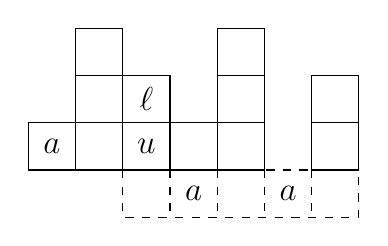
\begin{tikzpicture}[scale=.6]
\draw (0,0) -- (0,1) -- (5,1) -- (5,0) -- (0,0);
\draw (1,0) -- (1,3) -- (2,3) -- (2,0);
\draw (1,2) -- (3,2) -- (3,0);
\draw (4,0) -- (4,3) -- (5,3) -- (5,1);
\draw (4,2) -- (5,2);
\draw (6,0) -- (6,2) -- (7,2) -- (7,0) -- (6,0);
\draw (6,1) -- (7,1);
\draw[dashed] (2,0) -- (2,-1) -- (7,-1) -- (7,0) -- (2,0);
\draw[dashed] (3,0) -- (3,-1);
\draw[dashed] (4,0) -- (4,-1);
\draw[dashed] (5,0) -- (5,-1);
\draw[dashed] (6,0) -- (6,-1);
\node at (.5,.5) {\large $ a$};
\node at (2.5,.5) {\large $ u$};
\node at (2.5,1.5) {\large $ \ell$};
\node at (3.5,-.5) {\large $ a$};
\node at (5.5,-.5) {\large $ a$};
\node at (6.5,-.5) {\large $ $};
\end{tikzpicture}
\hspace*{2cm}
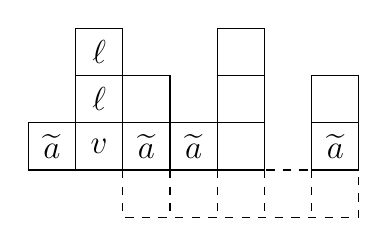
\begin{tikzpicture}[scale=.6]
\draw (0,0) -- (0,1) -- (5,1) -- (5,0) -- (0,0);
\draw (1,0) -- (1,3) -- (2,3) -- (2,0);
\draw (1,2) -- (3,2) -- (3,0);
\draw (4,0) -- (4,3) -- (5,3) -- (5,1);
\draw (4,2) -- (5,2);
\draw (6,0) -- (6,2) -- (7,2) -- (7,0) -- (6,0);
\draw (6,1) -- (7,1);
\draw[dashed] (2,0) -- (2,-1) -- (7,-1) -- (7,0) -- (2,0);
\draw[dashed] (3,0) -- (3,-1);
\draw[dashed] (4,0) -- (4,-1);
\draw[dashed] (5,0) -- (5,-1);
\draw[dashed] (6,0) -- (6,-1);
\node at (1.5,.5) {\large $v$};
\node at (1.5,1.5) {\large $\ell$};
\node at (1.5,2.5) {\large $\ell$};
\node at (.5,.5) {\large $\widetilde{a}$};
\node at (2.5,.5) {\large $\widetilde{a}$};
\node at (3.5,.5) {\large $\widetilde{a}$};
\node at (6.5,.5) {\large $\widetilde{a}$};
\end{tikzpicture}
\end{center}

\end{exam}

It will prove useful to have formulas for the action of $T_i$ on $E_\mu$, which is most simply expressed using diagram statistics.

\begin{lemm}\label{TiFormulas} We have the following formulas for the action of $T_i$ on the nonsymmetric Macdonald polynomials.
\begin{itemize} \item\hspace*{0mm}{\cite[(17)]{MR2405160}} If $\mu_{i}>\mu_{i+1}$ for some $1\le i<n$, then
\begin{align}
\label{E:T-on-E-up}
T_i E_\mu = E_{s_i(\mu)}-\frac{1-t}{1-q^{\ell_\mu(\square)+1}t^{a_\mu(\square)}}E_\mu
\end{align}
where $\square=(i,\mu_{i+1}+1)\in\dg(\mu)$.\\

\item\hspace*{0mm}[Proof in Appendices] If $\mu < \mu_{i+1}$, and $u=(i,\mu_{i}+1)$, then
\begin{equation} \label{decreasingT} T_iE_\mu = \frac{q^{\ell(u)+1}t^{a(u)}(1-t)}{1-q^{\ell(u)+1}t^{a(u)}}E_{\mu} - \frac{(t-q^{\ell(u)+1}t^{a(u)})(1-q^{\ell(u)+1}t^{a(u)+1})}{(1-q^{\ell(u)+1}t^{a(u)})^2} E_{s_i(\mu)},\end{equation}
where all arms and legs are in terms of the diagram of $s_i(\mu)$.\\

\item If $\mu_i = \mu_{i+1}$, then
\begin{equation}\label{simpledz} T_i E_\mu = t E_\mu.\end{equation}

\item Applying the above formulas, for any $w\in \Sn$,
\begin{equation}\label{span}
    T_w(E_\mu) \in \Lq \Spann \{ E_{w'(\mu)} \}_{w' \in \Sn}.
\end{equation}

\end{itemize}
\end{lemm}








\section{Properties of Partially-Symmetric Macdonald Polynomials}
\subsection{Stability}
The polynomials $\PP$ exhibit stability in the following sense. Considering the projection of polynomials in $\mathbb{K}[x_1,\dotsc, x_n]$,
\[ \pi_1(x_1^{\lambda_1} \dotsm x_n^{\lambda_n}) := \begin{cases} x_1^{\lambda_2} \dotsm x_{n-1}^{\lambda_n} &\text{ if } \lambda_1=0\\
0 &\text{ if } \lambda_1 > 0\end{cases}. \]

This is equivalent to setting $x_1 \mapsto 0$ and shifting the remaining indices down by 1.


\begin{prop} If $\lambda \in \Z_{\geq 0}^{n-k}$ is an $S_{[1,n-k]}$-dominant weight and $\gamma \in \Z_{\geq 0}^k$, then
\begin{align}\label{stability}\pi_1 P_{(\lambda,0\mid\gamma)} =  P_{(\lambda\mid\gamma)}.\end{align}\end{prop}

This is proved in~\cite{Lapointe} for the $m$-symmetric Macdonald Polynomials. An explicit computation in our notation can be found in~\cite{Dissertation}. As a result of that computation, with our choice of normalization, $P_{(\lambda|\gamma)}$ expands into the nonsymmetric Macdonald basis with the coefficient of $E_{\lambdamingamma}$ (and therefore due to triangularity the coefficient of $x^{\lambdamingamma}$ in the monomial basis) equal to 1.

\begin{rema}
    The partially-symmetric Macdonald polynomials form a basis for partially-symmetric polynomials in $\Lq[x_1, \dotsc, x_n]^{\Sn}$, which is a direct result of the fact that the $E_\mu$ form a basis for $\Lq[x_1,\dotsc,x_n]$.
\end{rema}


\subsection{Integral Form}\label{integralformsection}
The integral form partially symmetric Macdonald polynomial $\JJ=\JJ(x;q,t)$ is the scalar multiple
\[
\JJ = j_{(\lambda|\gamma)}P_{(\lambda|\gamma)}
\]
where
\[
\jj := \symmetricprod (1-q^{\ell_{\nu^-}(\square)}t^{\tilde{a}_{\nu^-}(\square) + 1}) \nonsymmetricprod(1-q^{\ell_{\nu^-}(\square) + 1}t^{a_{\nu^-}(\square) + 1}).
\]


In the definition of $j_{(\lambda|\gamma)}$, the products are taken over the symmetric and nonsymmetric parts of $\dg(\nu^-)$, respectively. That is, $\displaystyle{\symmetricprod}=\displaystyle{\prod_{\substack{(i,j) \in \nu^-\\ 1\leq i \leq n-k}}}$ and $\displaystyle{\nonsymmetricprod}=\displaystyle{\prod_{\substack{(i,j) \in \nu^-\\ n-k+1 \leq i \leq n}}}$.

\begin{rema}
    The integral form normalization agrees with the one in~\cite{Lapointe}.
\end{rema}

Before proving integrality of $\JJ$, we will break it down to pieces which we will prove individually. Fist, converting to the integral form of the nonsymmetric Macdonald polynomials found in~\cite[Eqn. (6.11)]{MR2348910}, denoted $\mathcal{E}_\nu$, and reorganizing the denominator, we get:

\begin{align*}\JJ &= \frac{\symmetricprod (1-q^{\legnumin}t^{\armonenumin + 1}) \nonsymmetricprod(1-q^{\legnumin + 1}t^{\armtwonumin + 1})}{  W^{n-k}_\lambda(t)} \\ &\hspace*{3cm} \cdot \frac{\Symm{\mathcal{E}_\nudom}}{\prod\limits_{\square \in \nu} \left(1-q^{\legnu+1}t^{\armtwonu +1} \right)} \\
&= \frac{\symmetricprod (1-q^{\legnumin}t^{\armonenumin + 1}) }{  \prod\limits_{\square \in d_{>1}(\lambda)} \left(1-q^{\legnu+1}t^{\armtwonu +1} \right)  } \cdot \frac{\nonsymmetricprod(1-q^{\legnumin + 1}t^{\armtwonumin + 1})}{\prod\limits_{\square \in \gamma} \left(1-q^{\legnu+1}t^{\armtwonu +1} \right)}   \\
&\hspace*{3cm} \cdot  \frac{\Symm{\mathcal{E}_{(\lambda \mid \gamma)}}}{W^{n-k}_\lambda(t)\prod\limits_{\square \in d_1(\lambda)} \left(1-q^{\legnu+1}t^{\armtwonu +1} \right)} \end{align*}

The middle products cancel immediately, since the ordering of the columns of $\lambda$ does not change the arm length of a box in $\gamma$. So this can be simplified to
\begin{equation}\label{simplifiedJ} \JJ = \frac{\symmetricprod (1-q^{\legnumin}t^{\armonenumin + 1}) }{  \prod\limits_{\square \in d_{>1}(\lambda)} \left(1-q^{\legnu+1}t^{\armtwonu +1} \right)  } \cdot  \frac{\Symm{\mathcal{E}_{(\lambda \mid \gamma)}}}{W^{n-k}_\lambda(t)\cdot \prod\limits_{\square \in d_1(\lambda)} \left(1-q^{\legnu+1}t^{\armtwonu +1} \right)}. \end{equation}

Then to complete the proof that $\JJ$ is integral, we will show that
\begin{align}\label{HHLpiece} \frac{\mathcal{E}_\nu}{\prod\limits_{ \square \in d_1(\lambda) }(1-q^{\legnu+1}t^{\armtwonu +1})} \in \Z[q,t][x_1, \dotsc, x_n],\end{align}
and also,
\begin{align}\label{coefficientpiece} \frac{\symmetricprod (1-q^{\legnumin}t^{\armonenumin + 1}) }{  \prod\limits_{\square \in d_{>1}(\lambda)} \left(1-q^{\legnu+1}t^{\armtwonu +1} \right)  } = \prod\limits_{\square \in d_{top}(\lambda^-)} (1-q^\legnumin t^{\armonenumin + 1}). \end{align}

We will make use of the combinatorial formula for the nonsymmetric Macdonald polynomials from~\cite{MR2405160} in order to prove~\eqref{HHLpiece}.
\begin{lemm}\label{redundancy} For any $\nu = \nudom$ where $\lambda$ has weakly decreasing entries 
\begin{equation}\label{integralfraction} \frac{\mathcal{E}_\nu}{\prod\limits_{ \square \in d_1(\lambda) }(1-q^{\legnu+1}t^{\armtwonu +1})} \in \Z[q,t][x_1, \dotsc, x_n]. \end{equation}
\end{lemm}
\begin{proof}
First, we will convert $\mathcal{E}_\nu$ back into its monic form $E_\nu$, so the lefthand side of~\eqref{integralfraction} is
\[\prod\limits_{\square \in d_{>1}(\lambda) }(1-q^{\legnu+1}t^{\armtwonu + 1}) \nonsymmetricprod(1-q^{\legnu+1}t^{\armtwonu + 1}) E_\nu.\]
Consider the combinatorial formula for $E_\nu$ given in ~\cite{MR2405160},
\[E_\nu = \sum\limits_{\substack{\sigma :\, \nu \to [n] \\ \text{nonattacking}}} x^\sigma q^{maj(\widehat{\sigma})}t^{coinv(\widehat{\sigma})} \prod\limits_{\substack{\square \in  \dg(\nu) \\ \widehat{\sigma}(\square) \neq \widehat{\sigma}(d(\square))}} \frac{1-t}{1-q^{\legnu+1} t^{\armtwonu+1}}.\]

The following definitions are taken directly from~\cite{MR2405160}. A filling $\sigma$ of the diagram $\nu$ is a function assigning a number $i\in \{1, \dotsc, n \} $ to each box in the diagram, which we will call the box's label. In this formula, $\dg(\nu)$ is the diagram of $\nu$ with no basement row. The term $d(\square)$ is the box immediately below $\square$, so the product is over every box in the diagram $\dg(\nu)$ which does not have a box below it with the same label. Then for a filling $\sigma$, the augmented filling $\widehat{\sigma}$ is a filling of the diagram $\dg(\nu) \cup \{ (i,0) \mid 1\leq i \leq n\}$ where $\widehat{\sigma}(i,0)=i$.

Two boxes $(i,j)$ and $(i',j')$ are said to be attacking if either,
\begin{itemize}
    \item The boxes are in the same row, i.e. $j = j'$, or
    \item The boxes are in adjacent rows and different columns, and the box in the lower row is to the right of the box in the higher row, i.e. the boxes are of the form $(i,j)$ and $(i-1,j')$ where $j' > j$.
\end{itemize}

A filling $\widehat{\sigma}$ of the augmented diagram is attacking if there is a pair of boxes in the augmented diagram which are attacking and which have the same label. And $\sigma$ is said to be a nonattacking filling of $\nu$ if the corresponding filling $\widehat{\sigma}$ of the augmented diagram is nonattacking. This means for $\sigma$ to be nonattacking, every pair of attacking boxes in the augmented diagram must have distinct values.

Now suppose $\sigma$ is a nonattacking filling of $\nu$. Since $\lambda$ is decreasing, every column $i$ in the $\lambda$ part of the augmented diagram where $\lambda_i \neq 0$ has boxes in the basement row and row 1. By assumption, each box $(i,0)$ contains the value $i$. So if we start filling in the boxes $(j,1)$ from left to right, the box $(1,1)$ is attacking every box $(j,0)$ where $j>1$, all the boxes to the right of column 1 in row 0. Continuing to the right, the box $(i,1)$ is attacking the boxes $(k,1)$ where $k<i$, and the boxes $(j,0)$ where $j>i$. Inductively, the boxes $(k,1)$ for $k<i$ are labeled $k$, and the boxes $(j,0)$ for $j>i$ are labeled $j$. So for the box to be nonattacking, $(i,1)$ must have label $i$. Then altogether, $(i,1)$ has label $i$ where $\lambda_i \neq 0$.

Finally, since $\sigma$ is nonattacking and must have the filling described above, every $\square = (i,1)$ 
from the first row of $\lambda$ must have the same label as the box $d(\square)$ below it, namely $i$.
Therefore, no box in the first row of $\lambda$ contributes to the product $\displaystyle{\prod\limits_{\substack{\square \in  \dg(\nu) \\ \widehat{\sigma}(\square) \neq \widehat{\sigma}(d(\square))}}} \frac{1-t}{1-q^{\legnu+1} t^{\armtwonu(\square)+1}}$. That means that the product, \[ \prod\limits_{\substack{\square \in \nu, \\ \square \notin d_1(\lambda) }}(1-q^{\legnu+1}t^{\armtwonu + 1}),\] or equivalently, \[\prod\limits_{\square \in d_{>1}(\lambda) }(1-q^{\legnu+1}t^{\armtwonu + 1}) \nonsymmetricprod(1-q^{\legnu+1}t^{\armtwonu + 1}),\] is sufficient to cancel all the denominators in the combinatorial formula for $E_\numin$. Therefore for this normalized form of the nonsymmetric Macdonald polynomials, \[\prod\limits_{\substack{\square \in \numin, \\ \square \notin d_1(\lambda^-) }}(1-q^{\legnumin+1}t^{\armtwonumin + 1}) E_\numin \in \mathbb{Z}[q,t][x_1,\dotsc,x_n].\qedhere\]
\end{proof}

\begin{lemm}\label{lambdalemma} If $\lambda$ is weakly decreasing,

\begin{equation}\label{lambdaequality}\frac{\symmetricprod (1-q^{\legnumin}t^{\armonenumin + 1}) }{  \prod\limits_{\square \in d_{>1}(\lambda)} \left(1-q^{\legnu+1}t^{\armtwonu +1} \right)  } = \prod\limits_{\square \in d_{top}(\lambda^-)} (1-q^\legnumin t^{\armonenumin + 1}).\end{equation}\end{lemm}

\begin{proof}
Let $w_{\lambda^-}\in \Sn$ be the shortest element such that $w_{\lambda^-}(\lambda)=\lambda^-$. Note that $w_{\lambda^-}$ does not change the ordering of columns of the same height relative to each other. Consider the boxes $u=(i,j)$ in $d_{>1}(\lambda)$ inside the diagram $\nudom$, and $u'=(w_{\lambda^-}(i),j-1)$, the box in $\nuantidom$ immediately below the box corresponding to $u$ after reversing $\lambda$. Since $u$ is not in the first row of $\lambda$, the box $u'$ appears in $\lambda^-$ and not in $d_{top}(\lambda)$.

We wish to show that $\widetilde{a}_\numin(u')=a_\nu(u)$ and $\ell_{\numin}(u')=\ell_\nu(u)+1$. The leg equality is immediate, since $u$ and $u'$ are in columns of the same height and $u'$ is one row below~$u$, and thus has one more leg than $u$.

To count the arms in $\widetilde{a}_\numin(u')$ and $a_\nu(u)$, consider the arms which are counted in the following cases:

\begin{itemize} \item Consider a column in $\gamma$ which could be counted in the right arms of $u$ and~$u'$. The same box is counted in the right arms, using the definitions of $a$ and $\widetilde{a}$, since $a_\nu(u)$ counts boxes in the row below~$u$, and $\widetilde{a}_\numin(u')$ counts boxes in the same row as $u'$, which are the same row, $j-1$. And the criterion for the box to be counted is the same in either case.

\item In $\lambda$ and $\lambda^-$, columns of height $\lambda_i$ are only counted if they are to the left of the box $u$ or $u'$ in their respective diagrams. Because those columns maintain the same order relative to each other, and left arms in $a$ and $\widetilde{a}$ are counted the same, $u$ and $u'$ have the same number of arms in those columns. 

\item Columns of height $\lambda_i-1$ appear to the right of $u$ in $\nu$ since $\lambda$ is weakly decreasing, and to the left of $u'$ in $\numin$ since $\lambda^-$ is weakly increasing. Then since the columns have fewer boxes than $\lambda_i$, these columns contribute to right right arm in $a_\nu(u)$. Similarly, the columns contribute to the left arm of in~$\widetilde{a}_\numin(u')$.

\item Columns of height greater than $\lambda_i$ or less than $\lambda_i-1$ do not contribute to either $\widetilde{a}_\numin(u')$ or $a_\nu(u)$.


\end{itemize}
Altogether, this implies that $\widetilde{a}_\numin(u') = a_\nu(u)$, and from that we can see that, \[1-q^{\ell_\numin(u')}t^{\widetilde{a}_\numin(u') + 1} = 1-q^{\ell_\nu(u)+1}t^{a_\nu(u) +1}.\]
This allows us to cancel most of the terms in the quotient on the left side of~\eqref{lambdaequality}. The terms coming from the boxes in $d_{>1}(\lambda)$ correspond to the terms from the boxes below them in $\lambda^-$. What's left in the numerator are terms from the top horizontal strip, $d_{top}(\lambda^-)$.
\end{proof}

Now to complete the proof that $\JJ$ is integral, it remains to show that the Poincar\'e polynomial $W^{n-k}_\lambda(t)$ is cancelled by the symmetrization of $E_\nu$.

\begin{thm}\label{Integrality}
If we expand $\displaystyle{\JJ = \sum_\mu c_{ \mu} x^\mu}$, with $\lambda$ weakly decreasing, then \mbox{$c_{ \mu} \in \Z[q,t]$} for any $\mu$.
\end{thm}

\begin{proof} 
Applying Lemma~\ref{lambdalemma} to~\eqref{simplifiedJ}, we can start by writing,
\begin{align*}  \JJ =  &\prod\limits_{\square \in d_{top}(\lambda^-)} (1-q^{\legnumin} t^{\armonenumin + 1}) \cdot \frac{1}{W^{n-k}_\lambda(t)} \\ & \hspace*{3cm}\cdot \Symm{\frac{\mathcal{E}_{(\lambda \mid \gamma)}}{\prod\limits_{\square \in d_1(\lambda)} \left(1-q^{\legnu+1}t^{\armtwonu +1} \right)}} . \end{align*}
 Looking at the symmetrizer and Poincar\'e polynomial, and decomposing each $w$ into $w=w'w''$ where $w'\in \Stabn$ and $w'' \in W^{\lambda}$ is the minimal length coset representative of $w\Stabn$ in $\Sn / \Stabn$, we get,
\[ \frac{1}{W^{n-k}_\lambda(t)} \sum\limits_{w\in \Sn} T_w = \frac{1}{\sum\limits_{w\in \Stabn(\lambda)} t^{\ell(w)}} \sum\limits_{w''\in W^\lambda}T_{w''} \sum\limits_{w'\in \Stabn}T_{w'}. \]
Then using~\eqref{simpledz}, the action of $T_{w'}$ is just multiplication by $t^{\ell(w')}$, and so,
\[ \frac{1}{W^{n-k}_\lambda(t)} \sum\limits_{w\in \Sn} T_w = \sum\limits_{w''\in W^\lambda}T_{w''}. \]
Finally, we can consider $\JJ$ as,
\[ \prod\limits_{\square \in d_{top}(\lambda^-)} (1-q^{\legnumin} t^{\armonenumin + 1})  \sum\limits_{w''\in W^\lambda}T_{w''}  \left(\frac{\mathcal{E}_{(\lambda \mid \gamma)}}{\prod\limits_{\square \in d_1(\lambda)} \left(1-q^{\legnu+1}t^{\armtwonu +1} \right)} \right).\]

Since the operators $T_i$ preserve $\Z[q,t][x_1,\dotsc,x_n]$, and from~\eqref{HHLpiece}, the function inside the symmetrizer is in $\Z[q,t][x_1,\dotsc,x_n]$, we conclude that $\JJ \in \Z[q,t][x_1,\dotsc,x_n]$.
\end{proof}

 By definition, $P_{\lambdagamma}$ has the symmetric and nonsymmetric Macdonald polynomials as special cases if we take $P_{(\lambda \mid \emptyset)}$ and $P_{(\emptyset \mid \gamma)}$ respectively. The formula for $\jj$ also specializes to the integrality constants of nonsymmetric Macdonald polynomials in~\cite{MR3443860}, and in the symmetric Macdonald polynomials in~\cite[section VI.8]{MR1427661}, so that
\[ j_{(\lambda \mid \emptyset)} P_{(\lambda \mid \emptyset)} = \mathcal{J}_\lambda \hspace{.5cm} \text{ and } \hspace{.5cm}  j_{(\emptyset \mid \gamma)} P_{(\emptyset \mid \gamma)} = \mathcal{E}_\gamma,\]
meaning $\JJ$ also has as special cases the integral forms of the symmetric and nonsymmetric Macdonald polynomials respectively. Additionally, because the diagram for $\jj$ is constructed with $\lambda$ rewritten in weakly increasing order, any extra 0 entries appended to $\lambda$ will not change the diagram, and thus $j_{(\lambda \mid \gamma)} = j_{(\lambda, 0 \mid \gamma)}$ for any $\lambda$ and~$\gamma$. Combining this with the stability of $\PP$, we have stability of $\JJ$ as well.

\subsection{Expansion into nonsymmetric Macdonald basis}
The nonsymmetric Macdonald polynomials form a basis for $\Lq[x_1, \dotsc, x_n]$, so every partially-symmetric Macdonald polynomial can be written in that basis. Additionally, we know from Lemma~\ref{TiFormulas} that for weakly decreasing partition $\lambda$ and composition $\gamma$,
\[ \Pn \in \Lq \Spann \{ E_{(w(\lambda) \mid \gamma)}\}_{w\in \Sn }.\]
It will prove useful in later computations to have formulas for the coefficients of that expansion in the nonsymmetric Macdonald basis.


\begin{prop}\label{Pexpansion}
In the expansion of $\PP$ into the nonsymmetric Macdonald basis,
\[ \PP = \sum_{\mu \in S_{[1,n-k]}(\lambda)} \fmu E_{\mugamma},\]
the coefficients satisfy the recurrence relation,
\begin{align} 
f_{\lambda^-,\lambdagamma} &= 1 \label{identity}\\
\fsimu &= \fmu \cdot \frac{t-\betaa}{1-\betaa},\label{recursion}\end{align}
if $s_i(\mu) < \mu$ and $u=(i, \mu_{i}+1)$.
\end{prop}
\begin{proof}
The identity~\eqref{identity} can be found using the formulas in Lemma~\ref{TiFormulas} and the triangularity of the nonsymmetric Macdonald polynomials. Let $\mu \in S_{[1,n-k]}(\lambda)$ be some weight such that $s_i(\mu)<\mu$ and define $u=(i,\mu_{i}+1)$. Since $\PP$ is invariant under the permutation $s_i$,

\[ T_i \PP = t \PP.\]
In the expansion into the nonsymmetric Macdonald basis, writing $\nu \sim \lambda$ to mean $\nu$ is a rearrangement of $\lambda$ (equivalently, $\nu \in S_{[1,n-k]}(\lambda)$),
\[ \sum_{\nu \sim \lambda} \fnuu T_i E_{\nugamma} = \sum_{\nu \sim \lambda} \fnuu t E_{\nugamma}.   \]
The recursive identity can be recovered by comparing the coefficients of $E_{(s_i(\mu) \mid \gamma)}$ on each side. On the right, we simply have $t\cdot f_{s_i(\mu),\lambdagamma}$. On the left, because $T_i E_{(\mu \mid \gamma)}$ is a linear combination of $E_{(\mu \mid \gamma)}$ and $E_{(s_i(\mu) \mid \gamma)}$, the only possible values of $\nu$ which contribute to the coefficient of $E_{(s_i(\mu) \mid \gamma)}$ are $E_\mugamma$ and $E_{(s_i(\mu) \mid \gamma)}$. Once again considering all arms and legs to be with respect to the diagram of $s_i(\mu)$, computing both possible contributions gives,
\begin{align*}
     &T_i E_{\mugamma} =  \frac{q^{\ell(u)+1}t^{a(u)}(1-t)}{1-q^{\ell(u)+1}t^{a(u)}} E_{\mugamma} +  \frac{(t-q^{\ell(u)+1}t^{a(u)})(1-q^{\ell(u)+1}t^{a(u)+1})}{(1-q^{\ell(u)+1}t^{a(u)})^2} E_{(s_i(\mu) \mid \gamma)}\\
    &T_i E_{(s_i(\mu)\mid \gamma)} =  E_{\mugamma} +  \frac{t-1}{1-q^{\ell(u)+1}t^{a(u)}} E_{(s_i(\mu)\mid \gamma)}
\end{align*}
Thus the coefficient of $E_{(s_i(\mu)\mid \gamma)}$ on the left side is,
\[ f_{s_i(\mu),\lambdagamma} \cdot \frac{t-1}{1-q^{\ell(u)+1}t^{a(u)}} + f_\mu  \cdot \frac{(t-q^{\ell(u)+1}t^{a(u)})(1-q^{\ell(u)+1}t^{a(u)+1})}{(1-q^{\ell(u)+1}t^{a(u)})^2}.\]
This must be equal to $t\cdot f_{s_i(\mu),\lambdagamma}$, which implies,
\[ f_{s_i(\mu),\lambdagamma} \left( t-\frac{t-1}{1-q^{\ell(u)+1}t^{a(u)}} \right) = f_\mu  \cdot \frac{(t-q^{\ell(u)+1}t^{a(u)})(1-q^{\ell(u)+1}t^{a(u)+1})}{(1-q^{\ell(u)+1}t^{a(u)})^2}.\]
After simplification, this is exactly~\eqref{recursion}.
\end{proof}


\begin{prop}
There is a closed formula for $\fmuu$,
\begin{equation}\label{closedform} \fmuu = t^{\ell(w_m)} \cdot \frac{\prod\limits_{\square \in (\lambda^- \mid \gamma)} \left( 1-q^{\ell_{(\lambda^- \mid \gamma)} (\square)+1} t^{a_{(\lambda^- \mid \gamma)} (\square)} \right)}{\prod\limits_{\square \in (\mu \mid \gamma)} \left( 1-q^{\ell_{(\mu \mid \gamma)} (\square)+1} t^{a_{(\mu \mid \gamma)} (\square)} \right) }, \end{equation}
where $w_m$ is the minimal length element in $S_{[1,n-k]}$ such that $w_m(\lambda^-)=\mu$.
\end{prop}
\begin{proof}
We will prove this by showing that the given formula for $\fmuu$ satisfies the recurrence relations in Proposition~\ref{Pexpansion}. The identity~\eqref{identity} is trivial. To show~\eqref{recursion}, suppose $s_i(\mu)<\mu$ for some $\mu \in S_{[1,n-k]}(\lambda)$. Let $w_m$ and $w'_m$ be the elements in $S_{[1,n-k]}$ of minimal length such that $w_m(\lambda^-)=s_i(\mu)$ and $w'_m(\lambda^-)=\mu$. We must now simplify
\begin{equation}\label{extrabox}\frac{f_{s_i(\mu),\lambdagamma}}{\fmuu} = t^{\ell(w_m)-\ell(w'_m)} \cdot \frac{\prod\limits_{\square \in (\mu \mid \gamma)} \left( 1-q^{\ell_{(\mu\mid \gamma)} (\square)+1} t^{a_{(\mu \mid \gamma)} (\square)} \right)}{\prod\limits_{\square \in (s_i(\mu) \mid \gamma)} \left( 1-q^{\ell_{(s_i(\mu) \mid \gamma)} (\square)+1} t^{a_{(s_i(\mu) \mid \gamma)} (\square)} \right) }. \end{equation}
Because $s_i(\mu)<\mu$, we have $\ell(w_m)-\ell(w'_m)=1$. Note that every box in the diagrams $\mugamma$ and $(s_i(\mu)\mid \gamma)$ has the same arms and legs in its corresponding diagram except one. The exception is the box $u$ whose coordinates in $s_i(\mu)$ are $(i,\mu_i+1)$, and the corresponding box $u'$ in $\mu$ with coordinates $(i+1,\mu_i+1)$. The boxes $u'$ and $u$ have the same number of legs. And $u$ has one more box in $s_i(\mu)$ in its arm than $u'$ in $\mu$, namely the box $(i+1,s_i(\mu)_{i+1})$. Thus we can write
\[ 1-q^{\ell_{(\mu\mid \gamma)} (u')+1} t^{a_{(\mu \mid \gamma)} (u')}=1-q^{\ell_{(s_i(\mu)\mid \gamma)} (u)+1} t^{a_{(s_i(\mu) \mid \gamma)-1} (u)}.\]
Now since every term from a box other than $u$ and $u'$ in~\eqref{extrabox} cancels, we are left with
\begin{align*} \frac{f_{s_i(\mu),\lambdagamma}}{\fmuu} &= t \cdot \frac{ 1-q^{\ell_{(\mu\mid \gamma)} (u')+1} t^{a_{(\mu \mid \gamma)} (u')}}{ 1-q^{\ell_{(s_i(\mu) \mid \gamma)} (u)+1} t^{a_{(s_i(\mu) \mid \gamma)} (u)} }\\
&= \frac{t-q^{\ell_{(s_i(\mu) \mid \gamma)} (u)+1} t^{a_{(s_i(\mu) \mid \gamma)} (u)}}{1-q^{\ell_{(s_i(\mu) \mid \gamma)} (u)+1} t^{a_{(s_i(\mu) \mid \gamma)} (u)}}.\end{align*}
Therefore the formula~\eqref{closedform} satisfies the recursive condition~\eqref{recursion}, and so the closed form we found is an equation for the coefficients $\fmuu$. \end{proof}







\section{Multiplication Rules}\label{ElementaryMultiplication}

Our next goal with the partially-symmetric Macdonald polynomials will be to find multiplication rules for $e_1[x_1,\dotsc, x_{n-k}] P_{\lambdagamma}$ in the basis $P_{\munu}$ of partially-symmetric Macdonald polynomials, where $e_1[x_1,\dotsc, x_{n-k}]$ is the elementary symmetric polynomial $x_1+ \dotsm + x_{n-k}$. After this is done, we will find a similar formula for $x_j \PP$ with $j>n-k$, so $x_j$ is a nonsymmetric variable, in a similar way. We refer to those coefficient formulas as Pieri rules.


	\subsection{Setup and notation}
From this point forward, we make the assumption that $0<k<n$. Because $e_1[x_1, \dotsc, x_{n-k}]$ and $\PP{\lambdagamma}$ are both symmetric in the first $n-k$ variables, so is their product. Additionally, since the two polynomials are homogeneous with degree 1 and $|\lambdagamma|$ respectively, their product will be a homogeneous polynomial with degree $|\lambdagamma|+1$. There is therefore an expansion,
\begin{equation}\label{finalexpansion} (x_{1} + \dots + x_{n-k}) \PP{\lambdagamma} =  \sum_{\substack{|\mueta| = |\lambdagamma| + 1 \\ \mu_1 \geq \, \dotsm \, \geq \mu_{n-k}}}  C^{\lambdagamma}_{\mueta} \PP{\mueta}.  \end{equation}

In order to compute the coefficients, we will be using similar methods to those used by Baratta in~\cite{MR2525842} to compute Pieri rules for the nonsymmetric Macdonald polynomials, in their case for $x_i E_\mu$. Because we will be making use of several of the formulas in that paper, we start by converting our notation into theirs.

The first difference in notation in our constructions and Baratta's is the indexing of the variables. In~\cite{MR2525842}, the variables are $z_j$ and are written in reverse order, so our $x_i$ corresponds to $z_{n+1-i}$. As a result, the vectors we have considered to this point, written as $\lambdagamma$, will be reversed, so our `symmetrized' variables appear at the end. For the element of maximum length $w_0 \in S_n$, the vector $\lambdagamma$ in our notation then corresponds to $w_0\lambdagamma$ in Baratta's.

The Hecke algebra operators $H_j$ are defined with identical relations to ours, with $H_j$ replacing $T_j$ in the braid relations and quadratic relations~\eqref{quadratic}. The action of $H_j$ is given by the equation,
\[ H_j = \frac{(t-1)z_j}{z_j-z_{j+1}} + \frac{z_j-tz_{j+1}}{z_j-z_{j+1}} s_j. \label{DLbaratta}\]
Then using the fact that $x^\mu = z^{w_0(\mu)}$, we find,
\[ T_i f(x_1, \dotsc, x_n) = H_{n-i}f(z_n, \dotsc, z_1).\]


Under these conventions, the nonsymmetric Macdonald polynomials $\EI{\lambdagamma}$ correspond to Baratta's $E_{w_0 \lambdagamma}(z;q^{-1},t^{-1})$. The inverted powers of $q$ and $t$ are a formality, since we only use that form of the nonsymmetric Macdonald polynomials as an intermediate step. For clarity, we will also denote the polynomials in Baratta's conventions with the dagger, so $\EBlong{\gammalambdamin}$. Specifically, they correspond by the equation,
\[ \EIlong{\lambdagamma}=\left[\EBlong{w_0\lambdagamma}\right]_{z_i \mapsto x_{n+1-i}}. \]
Where it is unambiguous, the argument $(z;q^{-1},t^{-1})$ will be suppressed. Using the Hecke algebra isomorphism mapping $T_i$ to $H_{n-i}$, we get the definition of the partially-symmetric Macdonald polynomials,
\[\PBlong{\gammalambdamin} := \frac{1}{W^{n-k}_{\lambda}(t)} \sum_{w\in S_{[k+1, n]}} H_w \EBlong{\gammalambdamin}.\]

Because the $H_w$ act the same as the corresponding $T_w$ in our symmetrizers, we will also write this as,
\[ \PB{\gammalambdamin} = \eplusB  \EB{\gammalambdamin} \hspace*{.5cm} \text{ or } \hspace*{.5cm} \PB{\gammalambdamin} = \ep \EB{\gammalambdamin}. \]

In cases where we need the expansion of $\PB{\gammalambdamin}$ as a $\mathbb{Q}(q,t)$-linear combination of the nonsymmetric Macdonald polynomials, we will write,
\[ \PB{\gammalambdamin}=\sum_{\nu \sim \lambda} \fnu \EB{\gammanu},\]
where the $\fnu$ is equal to $f_{\mu, \eta}$ in Proposition~\ref{Pexpansion} where $\nu$ is $\mu$ written in reverse order, and $\eta$ is $\gammalambdamin$ in reverse order.
    \subsection{Interpolation Polynomials}
The following definitions can be found in~\cite{MR2525842}. In order to derive Pieri-type formulas, we will be working with the interpolation nonsymmetric Macdonald polynomials. Begin with the eigenvalues associated with~$E_\nu^\dagger$,
\begin{equation}\label{eigenvalueformula} \overline{\nu}_i = q^{\nu_i} t^{-l'_\nu(i)}, \hspace*{.5cm} 1\leq i \leq n,\end{equation}
\[ l'_\nu(i) = \# \{j<i \mid \nu_j \geq \nu_i\} + \# \{j>i \mid \nu_j > \nu_i\}.\]
Let $\overline{\nu} = (\overline{\nu}_1, \dotsc, \overline{\nu}_n)$ be the vector whose entries are the corresponding eigenvalues. These eigenvalues can be used to define the interpolation nonsymmetric Macdonald polynomials, which are the unique polynomials (up to normalization) $\Estarlong{\nu}$ of degree $| \nu |$ which satisfy evaluation criteria,
\begin{align}\label{vanishing} \begin{cases}\Estar{\nu}(\overline{\mu}) = 0  \hspace*{.5cm}\text{if } \mu \neq \nu \text{ and } |\mu| \leq |\nu|\\
\Estar{\nu}(\overline{\nu}) \neq 0
\end{cases}\end{align}

By Theorem 3.9 in~\cite{MR1456318}, the top homogeneous component of $\Estar{\nu}$ is a constant multiple of the corresponding nonsymmetric Macdonald polynomial $\EB{\nu}$. We use this to choose a normalization,
\[\Estarlong{\nu} = \EBlong{\nu} + \sum_{|\mu| < |\nu|} h_{\mu,\nu} \EBlong{\mu}.  \]

With the normalization chosen, the nonzero evaluation has an explicit formula, given in Proposition 6 of~\cite{MR2525842}:
 \begin{equation}\label{Estarformula} E^*_{\nu}(\overline{\nu}) = \left( \prod_{i=1}^n \overline{\nu}_i^{\nu_i} \right) \prod_{\square \in \nu} (1-q^{-(\ell_\nu(\square)+1)} t^{-a_\nu(\square)}).\end{equation}


Thus define a $\mathbb{Q}(q,t)$-linear isomorphism $\Psi:\K[x_1, \dotsc, x_n] \to \K[x_1, \dotsc, x_k]$ which sends $\EBlong{\nu}$ to $\Estarlong{\nu}$. Note that the powers of $q$ and $t$ in the argument of the interpolation polynomials are again positive, so in our notation, $\EIlong{\nu}$ corresponds to $\Estarlong{w_0(\nu)}$.

The following lemmas will be useful when we look at the actions of the Hecke algebra on the interpolation polynomials.

\begin{lemm}\label{eigenvaluepermutations}
Let $\mu$ be a composition with its corresponding vector of eigenvalues $\overline{\mu}$. Then $s_i \overline{\mu} = \overline{s_i\mu}$ if and only if $\mu_i \neq \mu_{i+1}$.
\end{lemm}
\begin{proof}
This comes by comparing directly the $i$th and $(i+1)$st column eigenvalues.
 \end{proof}

\begin{lemm}\label{eigentwo}
Let $\mu$ be a composition with $\mu_n>0$. Then
\[\overline{(\mu_n-1, \mu_1, \dotsc, \mu_{n-1})} = (q^{-1} \overline{\mu}_n\, , \, \overline{\mu}_1\, , \, \dotsc\, , \overline{\mu}_{n-1}).\]
\end{lemm}
\begin{proof}
This is once again immediate from the eigenvalue definition.
\end{proof}



In Theorem 3.6 of~\cite{MR1456318}, the interpolation nonsymmetric Macdonald polynomials are proven to be simultaneous eigenfunctions of the commuting operators,
\[ \Xi_i := z_i^{-1} + z_i^{-1}H_i \dotsm H_{n-1} \Phi H_1 \dotsm H_{i-1},\]
where $\Phi$ is defined by
\[ \Phi = (z_n-t^{-n+1})\Delta,\]
\[ \Delta f(z_1, \dotsc, z_n) = f\left(\frac{z_n}{q}, z_1, \dotsc, z_{n-1}\right).\]
With these operators, we have
\[ \Xi_i \Estar{\nu}=(\overline{\nu}_i)^{-1} \Estar{\nu}.\]

Then define the following operators on the interpolation polynomials,
\[ Z_i := t^{-\binom{n}{2}} (z_i \Xi_i-1) \Xi_1 \dotsm \reallywidehat{\Xi_i} \dotsm \Xi_n,\]
where $\reallywidehat{\Xi_i}$ means $\Xi_i$ is not included in the list. 
The significance of $Z_i$ stems from a useful corollary in~\cite{MR2525842},
\begin{equation}\label{isomorphism} z_i \EBlong{\nu} = q^{|\nu|} \Psi^{-1} Z_i \Estarlong{\nu}.\end{equation}

    \subsection{Interpolation polynomial expansion}
We now begin with the computations that will lead to the desired Pieri formulas. First, following definitions from Baratta, define a modified version of the operators $Z_i$,
\[ \ZZ_i := H_i \dotsm H_{n-1} \Phi H_1 \dotsm H_{i-1}=z_i \Xi_i - 1. \]

With this definition, the definition of $Z_i$, and using commutativity of the $\Xi_j$, we have an identity,
\[ Z_i = t^{-\binom{n}{2}} \ZZ_i\, \Xi_i^{-1} \prod_{j=1}^n \Xi_j. \]

This form with the full product $\displaystyle{\prod_{j=1}^n \Xi_j}$ is useful since the product acts identically on all interpolation nonsymmetric Macdonald polynomials of the same degree.

\begin{lemm}
Let $\mu$ be a composition. Then $\displaystyle{\prod_{j=1}^n \Xi_j \Estar{\mu} = q^{-|\mu|} t^{\binom{n}{2}} \Estar{\mu}}$.
\end{lemm} \begin{proof} The eigenvalue of $\displaystyle{\prod_{j=1}^n \Xi_j}$ acting on $E^\dagger_{\mu}$ has a power of $q$ equal to $\displaystyle{-\sum_{i=1}^n \mu_i} = -|\mu|$, and a $t$ power equal to $\displaystyle{\sum_{j=1}^n l'_\nu(i) = \binom{n}{2}}$. Hence the eigenvalue associated with $\displaystyle{\prod_{j=1}^n \Xi_j}$ is $q^{-|\mu|} t^{\binom{n}{2}}$.
\qedhere
\end{proof}


Every nonsymmetric Macdonald polynomial in the expansion of $\PB{\gammalambdamin}$ has the same degree, so $\displaystyle{\prod_{j=1}^n \Xi_j}$ acts identically on each of those terms, and thus,


\[ \prod_{j=1}^n \Xi_j \PB{\gammalambdamin} = q^{-|\mu|}t^{\binom{n}{2}} \PB{\gammalambdamin}.\]

We also need the fact that $H_i$ acts the same on nonsymmetric Macdonald polynomials as their interpolation counterparts. This can be seen in~\cite[page 6]{MR2534801}. We have the relation,
\begin{equation}\label{Tiactthesame} H_i \EB{\nu} = \Psi^{-1} H_i \Estar{\nu} .\end{equation}

Now we have all the required pieces to set up the desired computation, beginning by using~\eqref{Tiactthesame} and the $\Lq$-linearity of $\Psi$ to pass $\Psi^{-1}$ through the symmetrizer, and then~\eqref{isomorphism} to move it through the sum of monomials. We also abbreviate $\eplusB$ to~$\ep$.
\begin{align*}
    (z_{k+1} + \dots + z_n) \PB{\gammalambdamin} &=  \left(\sum_{j=k+1}^n z_j \right) \eplusB \Psi^{-1} \Estar{\gammalambdamin}\\
     &=  \left(\sum_{j=k+1}^n z_j \right) \Psi^{-1} \ep \Estar{\gammalambdamin}\\
    &= q^{|\gammalambdamin|} \Psi^{-1} \left( \sum_{j=k+1}^n Z_j \ep \Estar{\gammalambdamin}\right)\\
    &= q^{|\gammalambdamin|}\Psi^{-1}  \left( \sum_{j=k+1}^n \left( t^{-\binom{n}{2}} \ZZ_j\, \Xi_j^{-1} \prod_{\ell=1}^n \Xi_\ell \right) \ep \Estar{\gammalambdamin}\right)\\
    &= \Psi^{-1} \left( \sum_{j=k+1}^n \left( \ZZ_j\, \Xi_j^{-1} \right) \ep \Estar{\gammalambdamin}\right)\\
    &= \Psi^{-1} \left( \sum_{j=k+1}^n \left( H_j \dotsm H_{n-1} \Phi H_1 \dotsm H_{j-1} \, \Xi_j^{-1} \right) \ep \Estar{\gammalambdamin}\right)   \end{align*}
Combining the above with~\eqref{finalexpansion}, we have
\begin{align*} \sum_{\substack{|\etamu| = |\lambdagamma| + 1 \\ \mu_1 \geq \, \dotsm \, \geq \mu_{n-k}}}  C^{\gammalambdamin}_{\etamu} &\PP{\etamu} = \\ \Psi^{-1} &\left( \sum_{j=k+1}^n \left( H_j \dotsm H_{n-1} \Phi H_1 \dotsm H_{j-1} \, \Xi_j^{-1} \right) \ep \Estar{\gammalambdamin}\right). \end{align*}

Then taking $\Psi$ of both sides and once again using~\eqref{Tiactthesame} on the left side,
\begin{equation}\label{bothsides}  \sum_{\substack{|\etamu| = |\lambdagamma| + 1 \\ \mu_1 \geq \, \dotsm \, \geq \mu_{n-k}}}  C^{\gammalambdamin}_{\etamu} e^+ \Estar{\etamu} = \sum_{j=k+1}^n \left( H_j \dotsm H_{n-1} \Phi H_1 \dotsm H_{j-1} \, \Xi_j^{-1} \right) \ep \Estar{\gammalambdamin}.\end{equation}
This is the equation we will use to compute $C_{\etamu}^{\gammalambdamin}$. The first simplification will be using the relation (see ~\cite{MR1456318}),
\[ H_i \Xi_{i+1}^{-1} = \Xi^{-1}_i \overline{H_i},\]
where 
\[\overline{H_i} := \frac{(t-1)z_{i+1}}{z_i-z_{i+1}} + \frac{z_i-tz_{i+1}}{z_i-z_{i+1}} s_i.\]
This $\overline{H_i}$ is almost the inverse of $H_i$, but instead their multiplication is given by,
\[H_i \overline{H_i} = t.\] Importantly, if $f=s_i f$, then $\overline{H_i} f = f$. In particular, this means for $i\geq k+1$,
\[ \overline{H_i} \PB{\gammalambdamin} = \PB{\gammalambdamin}.\]
Now continuing with our calculations,
\begin{align*}
   \sum_{\substack{|\etamu| = |\lambdagamma| + 1 \\ \mu_1 \geq \, \dotsm \, \geq \mu_{n-k}}}  C^{\gammalambdamin}_{\etamu} &e^+ \Estar{\etamu}  =  \sum_{j=k+1}^n  H_j \dotsm H_{n-1} \Phi H_1 \dotsm H_{j-1} \, \Xi_j^{-1} \ep \Estar{\gammanu}\\  
    &=  \sum_{j=k+1}^n  H_j \dotsm H_{n-1} \Phi H_1 \dotsm H_{k} \, \Xi_{k+1}^{-1}  \ep \Estar{\gammanu}\\
    &= \sum_{j=k+1}^n H_j \dotsm H_{n-1} \Phi H_1 \dotsm H_{k} \, \Xi_{k+1}^{-1} \sum_{\nu \sim \lambda} \fnu \Estar{\gammanu} \\
    &=  \sum_{\nu \sim \lambda} \fnu  \sum_{j=k+1}^n H_j \dotsm H_{n-1} \Phi H_1 \dotsm H_{k} \, \Xi_{k+1}^{-1} \Estar{\gammanu}
\end{align*}



Note that the way we have written the sum on the lefthand side, with $\mu$ weakly decreasing, guarantees no two nonsymmetric Macdonald polynomials in the sum symmetrize to the same partially-symmetric Macdonald polynomial, so the coefficients $C_{\etamu}^{\gammalambdamin}$ are well-defined.

    \subsection{Expansion Support}
In this section, we will determine the weights which appear with nonzero coefficients in the Pieri expansion. This process serves the dual purpose of setting up the final computation for the coefficients. The following result identifies all possible coefficients which could appear, and we will show in Corollary~\ref{support} that every such coefficient is nonzero.
\begin{prop}\label{expansion}
In the Pieri expansion,
\[ (z_{k+1} + \dots + z_n)\PB{\gammalambdamin} = \sum_{\substack{|\etamu| = |\gammalambdamin| + 1 \\[1mm] \mu^-_1 \leq \, \dotsm \, \leq \mu^-_{n-k} }} C^{\gammalambdamin}_{\etamu} \PB{\etamu}, \]
we have $C^{\gammalambdamin}_{\etamu}\neq 0$ only if, for some $I_1=\{t_1, \dots, t_r\} \subseteq [1,k]$ with $t_1 < \, \dotsm \, < t_r$, and $\nu \in S_{n-k}(\lambda^-)$, the nonsymmetric part $\eta$ is
\begin{align*}
    &\eta_i = \gamma_i \hspace*{.55cm}\text{ if } i\notin I_1\\
    &\eta_{t_j}=\gamma_{t_{j+1}} \text{ for } 1\leq j \leq r \text{ where } \gamma_{t_{r+1}} = \nu_1,
\end{align*}
and the symmetric part $\mu^-$ satisfies
\begin{align*}
    (\mu_1^-, \dotsc, \mu_{n-k}^- ) \in S_{n-k}(\nu_2, \dotsc, \nu_{n-k}, \gammanu_{t_1}+1).
\end{align*}
In the case that $I_1 = \emptyset$, we have $\eta = \gamma$ and $\gammanu_{t_1} := \nu_1$.
\end{prop}
\begin{proof}

We first must analyze the actions of $H_i$ and $\Phi$ on interpolation nonsymmetric Macdonald polynomials. To simplify the formula for the $H_i$, define some functions, following~\cite{MR2525842},
\[ a(x,y) := \frac{(t-1)x}{x-y}, \hspace*{.5cm} b(x,y) := \frac{x-ty}{x-y}.\]
Then write $H_i = a(z_i,z_{i+1}) + b(z_i,z_{i+1}) s_i$. To continue, note that in the full expression,
\begin{equation}\label{rightside}\sum_{\nu \sim \lambda} \fnu\left( \sum_{j=k+1}^n \left( H_j \dotsm H_{n-1} \Phi H_1 \dotsm H_{k} \, \Xi_{k+1}^{-1} \right)  \Estar{\gammanu}\right),\end{equation}
because $\Xi^{-1}_{k+1}$ is acting on an interpolation polynomial, it acts as a constant eigenvalue which depends only on $\gammanu$, and does not impact the support. So we are evaluating the resulting polynomials in the expansion of $H_j \dots H_{n-1} \Phi H_1 \dots H_k \Estarlong{\gammanu}$. 
Expanding all of the $H_i$ operators and $\Phi$, we obtain
\begin{align*} &  [a(z_j,z_{j+1})+b(z_j,z_{j+1}) s_j] \dotsm [a(z_{n-1},z_n)+b(z_{n-1},z_n) s_{n-1}]\,    (z_n-t^{-n+1})\Delta \, \\& \hspace*{1cm} \cdot [a(z_1, z_2)+b(z_1,z_2) s_1] \dotsm [a(z_k,z_{k+1}) + b(z_k,z_{k+1})s_k] \, \Estarlong{\gammanu}.
\end{align*}



Since $s_i$ permutes the variables $z_i$ and $z_{i+1}$, we have that the action of the simple reflections is $s_i\Estarlong{\gammanu} = \Estar{\gammanu}(s_i(z);q,t)$. While this does not change the index $\gammanu$, the argument $s_i(z)$ means this is no longer an interpolation nonsymmetric Macdonald polynomial. Finding a term after expanding the above product corresponds to choosing either $a(z_i,z_{i+1})$ or $b(z_i,z_{i+1}) s_i$ from each bracketed pair. In this way, choose two sets $I_1=\{t_1< \, \dotsm \, < t_r\} \subseteq [1,k]$ and $I_2=\{v_1< \, \dotsm \, < v_s\} \subseteq [j,n-1]$ so that if $i\in I_1$, we choose $a(z_i,z_{i+1})$, and if $i\notin I_1$, we choose $b(z_i,z_{i+1})s_i$, and the same for $I_2$. We will write
\[ w_{I_1} := \shatproduct \]
to mean the full product $s_1 \dotsm s_k$ with the simple reflections with a hat removed. Let~$p_{I_1}(z)$ be the coefficient obtained from the terms in
\[ \Delta [a(z_1, z_2)+b(z_1,z_2) s_1] \dotsm [a(z_k,z_{k+1}) + b(z_k,z_{k+1})s_k] = \sum_{I_1\subseteq [1,k]} p_{I_1}(z) \Delta w_{I_1}.\]
Similarly, define the permutation
\[w_{I_2} := s_j \dotsm \widehat{s_{v_1}} \dotsm \widehat{s_{v_s}} \dotsm s_{n-1} \]
Let $p_{2}(z)$  be the coefficient obtained from terms in
\begin{align*} [a(z_j,z_{j+1})+b(z_j,z_{j+1}) s_j] \dotsm [a(z_{n-1},z_n)+b(z_{n-1},z_n) s_{n-1}] &(z_n-t^{-n+1})\\ &=\sum_{I_2\subseteq[j,n-1]}p_2(z)w_{I_2}.\end{align*}
Notice that the $(z_n-t^{-n+1})$ term is part of $p_2$. Additionally, we call this $p_2$ rather than $p_{I_2}$ because in later computations, we will find that the Pieri coefficients do not depend on $I_2$. Using these definitions, we can write an expansion of $\displaystyle{H_j \dotsm H_{n-1} \Delta H_1 \dotsm H_k  \Estarlong{\gammanu}}$ as
\begin{equation}\label{Expandedright}
      \sum\limits_{\substack{I_1 \subseteq [1,k] \\ I_2 \subseteq [j, n-1]}} p_{I_1}(z) \cdot p_2(z)  \cdot \left( s_j \dotsm \widehat{s}_{v_1} \dotsm \widehat{s}_{v_s} \dotsm s_{n-1}\Delta \shatproduct \right) \Estar{\gammanu}(z), \end{equation}
or more succinctly as
   \[ \sum\limits_{\substack{I_1 \subseteq [1,k] \\ I_2 \subseteq [j, n-1]}} p_{I_1}(z) \cdot p_2(z)  \cdot \Estar{\gammanu}(I_2(I_1(z))),
\]
where $I_1(z)$ and $I_2(z)$ are defined by
\begin{align} \label{Ione}&(I_1(z))_m := \begin{cases} z_m  &\text{ if } m\notin I_1 \text{ and } m \leq k \\
z_{t_{\ell-1}} \hspace*{.5cm} &\text{ if } m=t_\ell \text{ and } \ell \neq 1\\
q^{-1} z_n &\text{ if } m=t_1, \text{ or } r=0 \text{ and }m=k+1 \\
z_{t_r} &\text{ if } m=k+1 \text{ and } r\neq 0\\
z_{m-1} &\text{ if } m > k+1 \end{cases}\\[5mm]
\label{Itwo}& (I_2(z))_m := \begin{cases} z_m  &\text{ if } m\leq k \\
z_{m+1} \hspace*{.5cm} &\text{ if } m-1 \notin I_2, \text{ and } k+1 \leq m \leq n-1\\
z_{j} &\text{ if } m=v_1+1\\
z_{v_{i-1}+1} &\text{ if } m=v_i+1 \text{ and } i \geq 2\\
z_{v_s +1} &\text{ if } m=n, \text{ and if } s=0, \text{ then } v_s+1=j \end{cases}.\end{align}




The actions of $I_1$ and $I_2$ on the indices of the variables $z_i$ can be described as products of disjoint cycles, along with $\Delta$, by considering the whole permutation as follows in cyclic notation:
\[ s_j \dotsm \widehat{s}_{v_1} \dotsm \widehat{s}_{v_s} \dotsm s_{n-1}\Delta \shatproduct \]
\[ = (j \dots v_1) (v_1+1 \dots v_2) \dotsm (v_s+1 \dots n) \Delta (1 \dots t_1) (t_1+1 \dots t_2) \dotsm (t_r+1 \dots k+1).\]
This whole product can almost be combined into one long cycle,
\[ (v_s+1, v_{s-1}+1, \dots, v_1+1, j, j-1, \dots, k+2, k+1, t_r, t_{r-1}, \dots, t_1).\]
However, the cycling of $t_1$ to $v_s+1$ is special, since $I_2(I_1(z_{t_1})) = q^{-1} z_{v_s+1}$.

It is easier to work with the compositions $\gammanu$ than the lists of eigenvalues $\overline{(\eta \mid \mu)}$, so we would like to find an action $\dI$ for which 
\[\dI \gammanu=(\eta \mid \mu) \quad \text{ if and only if } \quad  I_2\left(I_1\left(\overline{(\eta \mid \mu)}\right) \right) = \overline{\gammanu}.\] The $I$ in $\dI$ should be thought of as $I = I_1 \cup I_2$. The following definition of $d_I$ is derived by repeated application of Lemma~\ref{eigenvaluepermutations} and one application of Lemma~\ref{eigentwo}. Note that the hypothesis in Lemma~\ref{eigenvaluepermutations} that $\mu_i \neq \mu_{i+1}$ means the property above only holds if $I_1$ and $I_2$ do not include the permutation $s_i$ if it would permute two columns of the same height. For now we take this for granted, but we will see in Lemma~\ref{comaximality} that we are only interested in $I_1$ which have this property, and the same will be shown explicitly for $I_2$ in the proof of Theorem~\ref{Pieriformula} when uniqueness of $I_2$ is established.

Assuming $I_1 \neq \emptyset$, the following definition of $\dI$ satisfies this property, and the horizontal bar separates the nonsymmetric and symmetric parts of $\dI\gammanu$:

\[ (\dI\gammanu)_m := \left\{\begin{tabular}{l l} $ \left.\begin{array}{l l} \gammanu_m  &\text{ if } m\leq k \text{ and } m\notin I_1 \\
\gammanu_{k+1} \hspace*{.7cm} &\text{ if } m=t_r\\
\gammanu_{t_{i+1}} &\text{ if } m=t_i \text{ and } i\neq r\end{array} \hspace{2cm} \right\} \, m \leq k$ \\
\underline{\hspace{9.5cm}}\\[2mm] $\left.\begin{array}{l l} \gammanu_{m+1} &\text{ if } k+1 \leq m < j\\
\gammanu_m &\text{ if } m>j \text{ and } m-1\notin I_2\\
\gammanu_{v_1+1} &\text{ if } m=j \text{ and } s\neq 0\\
\gammanu_{v_{i+1}+1} &\text{ if } m=v_i+1 \text{ and } 1 \leq i < s\\
(\gammanu_{t_1}) + 1&\text{ if } m=v_s+1 , \text{ or }  s=0 \text{ and } m = j \hspace*{0cm} \end{array} \right\} \, m \geq k+1 $ \end{tabular}  \right.\\[1mm]\]

If $I_1 = \emptyset$, the entry $(\gammanu_{t_1})+1$ in the last row should be replaced by \mbox{$(\gammanu_{k+1})+1$}. The constructions so far allow us to compute the partially-symmetric Macdonald polynomials which appear in the Pieri expansion, by considering evaluations of~\eqref{rightside}. First, we rewrite that equation using the operator expansions we have found:
\begin{equation}\label{newrightside}
    \sum_{\nu \sim \lambda} \fnu\left( \sum_{j=k+1}^n    \sum\limits_{\substack{I_1 \subseteq [1,k] \\ I_2 \subseteq [j, n-1]}} p_{I_1}(z) \cdot p_2(z)  \cdot \Estar{\gammanu}(I_2(I_1(z))) \right).
\end{equation} If we evaluate the expression at $z=\overline{\etamu}$, by the vanishing properties of the interpolation polynomials, we only get a nonzero term if $I_2\left( I_1 \left( \overline{\etamu} \right) \right) = \overline{\gammanu}$. So equivalently, this vanishes unless $\etamu = d_I\gammanu$ for some sets $I_1$ and $I_2$. From the definition of $d_I$, this happens when $\eta$ satisfies
\begin{align}
    &\eta_i = \gamma_i \hspace*{.55cm}\text{ if } i\notin I_1 \label{part1}\\
    &\eta_{t_j}=\gamma_{t_{j+1}} \text{ for } 1\leq j \leq r \text{ where } \gamma_{t_{r+1}} = \nu_1\label{part2}
\end{align}
and $\mu^-$ has
\begin{align}
    (\mu_1^-, \dotsc, \mu_{n-k}^- ) \in S_{n-k} (\nu_2, \dotsc, \nu_{n-k}, \gammanu_{t_1}+1).\label{part3}
\end{align}
Again we have that if $I_1 = \emptyset$, then $t_1$ should be considered as $k+1$. 

Then take the formula found earlier,
\begin{align*}   \sum_{\substack{|\etamu| = |\lambdagamma| + 1 \\ \mu_1 \geq \, \dotsm \, \geq \mu_{n-k}}}  C^{\gammalambdamin}_{\etamu} &e^+ \Estar{\etamu}  \\ &=  \sum_{\nu \sim \lambda} \fnu  \sum_{j=k+1}^n  H_j \dotsm H_{n-1} \Phi H_1 \dotsm H_{k} \, \Xi_{k+1}^{-1}  \Estar{\gammanu}.\end{align*}

Due to~\eqref{newrightside}, the right side vanishes when evaluated at $\overline{\etamu}$ unless $\etamu$ meets the above criteria. We know from~\eqref{Tiactthesame} that $e^+ \Estar{\etamu}$ expands in the same way as $ \PB{\etamu}$. So the left side must also vanish for $\etamu$ which don't meet those conditions. Because both sides are $\K$-linear combinations of interpolation polynomials,  using~\eqref{vanishing}, the only possible $\Estar{\etamu}$ which can appear with nonzero coefficients on the left are indexed by those same nonvanishing $\etamu$.

The order of $\mu^-$ is unimportant, since any permutation of $\mu^-$ contributes to the same $\PB{\etamu}$. Altogether, we conclude that the $\PB{\etamu}$ which appear in the expansion of $(z_{k+1} + \dotsm + z_{n})\PB{\gammanu}$ are those which satisfy~\eqref{part1},~\eqref{part2}, and~\eqref{part3}. \qedhere \end{proof}



 With this all constructed, we make the following notes:
\begin{itemize}
    \item The action of $\dI$ increases the height of exactly one column, which is found in $\mu^-$.
    \item Because $I_2$ permutes only the entries with positions in $[k+1,n]$, which will all symmetrize to the same partially-symmetric Macdonald polynomial, the action of $I_2$ does not change which terms appear as basis elements in the Pieri expansion.
\end{itemize}

We can now restrict the possible subsets $I_1$ which contribute to the Pieri-type coefficient formula.

\begin{lemm}\label{comaximality}Let $(\eta \mid \mu)$ be a composition such that $\overline{\gammanu} = I_2\left( I_1 \left(\overline{(\eta \mid \mu)} \right)\right)$ for some composition $\gammanu$ and sets $I_1\subseteq [1,k]$ and $I_2 \subseteq [j,n-1]$. Then the $I_1$ and $I_2$ which satisfy that equation are unique.
\end{lemm}
\begin{proof}
This is a consequence of Lemma~\ref{eigenvaluepermutations}, and is proved in~\cite[proof of Lemma~4.3] {MR1456318}.
\end{proof}

We will work more with $I_2$ in the proof of Theorem~\ref{Pieriformula}, but for now we define $I_1$ which is the unique set in the lemma above.


\begin{defi}\label{maximality}
We call $I_1$ maximal with respect to $(\gamma \mid \nu)$ and $I_2$ if there is some $(\eta \mid \mu)$ for which $\overline{(\gamma \mid \nu)} = I_2 \left( I_1 \left( \overline{(\eta \mid \mu)} \right)\right)$.
\end{defi}
In explicit terms, $I_1$ is maximal with respect to $\gammanu$ and if it satisfies:
\begin{enumerate}
    \item $\gamma_i \neq \gamma_{t_1}$ for all $i< t_1$, and if $I_1=\emptyset$, consider $\gammanu_{t_1} := \nu_1$ \item $\gamma_i \neq \gamma_{t_{u+1}}$ for all $t_u+1 \leq i \leq t_{u+1}-1$
\end{enumerate}


Note that the set $I_1$ which satisfies the above crieria is called \textit{comaximal} with respect to $\gammanu$ in~\cite{MR2525842}. We also omit the reference to $I_2$ in maximality where it is not needed. We will show after computing the coefficients $\pIone$ and $\pItwo$ that for a particular choice of $I_2$ and maximal $I_1$, the coefficient $C^{\gammalambdamin}_{\etamu}$ is nonzero. Finally, we give notation for the support set.

\begin{defi}
Define $\MM$ to be the set of compositions which appear in Proposition~\ref{expansion},
\begin{align*} \MM := \{\, \etamu \hspace*{.2cm} \Big| \hspace*{.2cm} \dI &\gammanu = \etamu \text{ for some } \nu \in S_{n-k}(\lambda^-), \text{ some maximal} \\ & \text{set } I_1 \text{ and some } \mu^- \in S_{n-k}(\nu_2, \dotsc, \nu_{n-k}, \gammanu_{t_1}+1)\} .\end{align*}
\end{defi}


\begin{exam}
    In the support of $(z_4+z_5)\PB{(2,0,1 \mid 1,2)}$, we can have $\nu_1=1$ or $\nu_1=2$. The following are all maximal $I_1$ and resulting composition $\etamu$ for each of these.

    \begin{center} 
        $\nu_1=1$ \quad\begin{tabular}{c|c} $I_1$ & $\etamu$ \\ \hline
        $\{1,2,3\}$ & $(0,1,1 \mid 2,3)$  \\
        $\{1,3\}$ & $(1,0,1 \mid 2,3)$ \\
        $\{2,3\}$ & $(2,1,1 \mid 1,2)$\\
        $\{3\}$ & $(2,0,1 \mid 2,2)$\end{tabular} \qquad $\nu_1=2$ \quad\begin{tabular}{c|c} $I_1$ & $\etamu$ \\ \hline
        $\{1,2,3\}$ & $(0,1,2 \mid 1,3)$  \\
        $\{1,2\}$ & $(0,2,1\mid 1,3)$ \\
        $\{2,3\}$ & $(2,1,2 \mid 1, 1)$\\
        $\{1,3\}$ & $(1,0,2\mid 1,3)$\\
        $\{1\}$ & $(2,0,1 \mid 1, 3)$\\
        $\{2\}$ & $(2,2,1 \mid 1,1)$\\
        $\{3\}$ & $(2,0,2 \mid 1,2)$\end{tabular}
    \end{center}
\end{exam}

    \subsection{Pieri coefficient computation}\label{Piericomputation}
Let us return to the equation which we will use to determine the Pieri coefficients:
\begin{align}\label{evaluatethis}\sum_{|\etamu| = |\gammalambdamin| + 1} &C^{\gammalambdamin}_{\etamu} \ep \Estar{\etamu}(z)\nonumber \\ = &\sum_{\nu \sim \lambda} \fnu \left( \sum_{j=k+1}^n \left( H_j \dotsm H_{n-1} \Phi H_1 \dotsm H_{k} \, \Xi_{k+1}^{-1} \right)  \Estar{\gammanu}(z)\right)\end{align}

Our approach will be to evaluate both sides at a particular value for $z$, and solve the equation for $C_{\etamu}$. First, use the expansion of $\ep \Estar{\etamu}(z)$ into nonsymmetric interpolation polynomials,
\begin{align}\label{evaluationpoint}\sum_{\etamu}  C^{\gammalambdamin}_{\etamu} &\sum_{\mu' \sim \mu} \gmuprime \Estar{\etamuprime}(z)\nonumber\\
&= \sum_{\nu \sim \lambda} \fnu \left( \sum_{j=k+1}^n \left( H_j \dotsm H_{n-1} \Phi H_1 \dotsm H_{k} \, \Xi_{k+1}^{-1} \right)  \Estar{\gammanu}(z)\right)\end{align}

By the vanishing property of interpolation polynomials, evaluating at a vector of eigenvalues $\overline{\etamuprime}$ will cause all but one term to vanish on the left side. We will choose a particular value of $\mu'$ that we call $\mutilde$ which simplifies our remaining computations. Starting with a vector $\gammalambdamin$, we begin by choosing some $\etamu$ in $\MM$, which determines a unique $I_1$ that is maximal with respect to $\gammalambdamin$. Notice that going from $\gammalambdamin$ to $\etamu$, exactly one column height from $\lambda^-$ is removed, and one column has its height increased in the creation of $\mu^-$. This can be read directly from $\lambda^-$ and $\mu^-$ unless $\lambda^-=\mu^-$. If this is the case, both the removed $\lambda^-$ column and the increased $\mu^-$ column have a height $\gamma_i$ where $i$ is the largest value for which $\gamma_i \neq \eta_i$.

Then for the choice of which $\mutilde$ to use in the evaluation, we require all columns with the same height as the increased column in $\mu^-$ to be at the beginning of the vector. The remaining entries are chosen to be weakly decreasing. As a consequence of the choice of $\mutilde$, we will see later that there is only one contributing $\nu$ in the sum indexed by $\nu$. We call this special composition $\lambdatilde$, which is given by
\[(\lambdatilde_1,  \dotsc, \lambdatilde_{n-k}) = (\eta_{t_r}, \mutilde_2, \dotsc, \mutilde_{n-k}) \]
if $I\neq \emptyset$, and if $I = \emptyset$,
\[ (\lambdatilde_1, \dotsc, \lambdatilde_{n-k}) = (\mutilde_1-1, \mutilde_2, \dotsc, \mutilde_{n-k}).\]
It is useful to define a value,
 \[\mIone := |\{ 1\leq i \leq n-k \mid \, \mutilde_i = \mutilde_1  \}|-1. \]
This is the same as the number of entries in $(\lambdatilde_2,\dotsc, \lambdatilde_{n-k})$ which are the same height as the newly increased column. We now have enough to write the coefficients in the Pieri expansion.

\begin{thm}\label{Pieriformula}
The product $e_1[z_{k+1},\dotsc, z_n] \PB{\gammalambdamin}$ can be written as a sum of partially-symmetric Macdonald polynomials with the formula,
\[ (z_{k+1} + \dotsm + z_n)\PB{\gammalambdamin} = \sum_{\etamu \in \MM} C^{\gammalambdamin}_{\etamu} \PB{\etamu},\]
where
\[C^{\gammalambdamin}_{\etamu} = \frac{f_{\lambdatilde,\lambdagamma}}{\fmutilde} \cdot \overline{\gammalambdatilde}_{k+1} \cdot p_{I_1} \cdot p_{2}\cdot \frac{\Estar{\gammalambdatilde}\left(\overline{\gammalambdatilde} \right)}{\Estar{\etamutilde} \left( \overline{\etamutilde}\right)}, \]
 the symmetric parts $\mutilde$ and $\lambdatilde$ are those described above, the set $I_1=\{t_1 < \, \dotsm \, < t_r\}$ is maximal with respect to $\gammalambdatilde$, $m := \mIone$, and $p_{I_1}$ and $p_{2}$ are given by
\begin{align*}
    p_{I_1}     &= \frac{(t-1)q^{-1} \overline{\mutilde}_{m+1}}{q^{-1} \overline{\mutilde}_{m+1}-\overline{\eta}_{t_1}} \prod_{u=1}^{r-1} \left(\frac{(t-1) \overline{\eta}_{t_u}}{ \overline{\eta}_{t_u}-\overline{\eta}_{t_{u+1}}}\right)  \prod_{j=1}^{t_1-1} \left( \frac{q^{-1} \overline{\mutilde}_{m+1} - t \overline{\eta}_j}{q^{-1} \overline{\mutilde}_{m+1} -  \overline{\eta}_j} \right) \\ & \hspace*{8cm} \cdot \prod_{u=1}^{r} \prod_{j=t_u+1}^{t_{u+1}-1}  \left(\frac{\overline{\eta}_{t_u} - t \overline{\eta}_j}{ \overline{\eta}_{t_u} -  \overline{\eta}_j} \right)\\[3mm]
    p_{2} &= \frac{1-t^{m+1}}{1-t}\cdot (\overline{\mutilde}_{m+1} - t^{-n+1}) \cdot \prod_{j=m+2}^{n-k} \frac{\overline{\mutilde}_{m+1} - t \cdot \overline{\mutilde}_j}{\overline{\mutilde}_{m+1} - \overline{\mutilde}_j}.
\end{align*}
\end{thm}
\begin{proof}The remainder of the derivation proceeds by evaluating both sides of~\eqref{evaluatethis} at $\overline{\etamutilde}$. Because the sums in the left side were constructed to have no overlapping terms, evaluation of the left side of the equation gives
\[ \sum_{\etamu} C^{\gammalambdamin}_{\etamu} \sum_{\mu' \sim \mu} f_{\mu',\etamu} \cdot \Estar{\etamuprime}\left(\overline{(\eta \mid \widetilde{\mu})}\right)= C^{\gammalambdamin}_{\etamu} \, \gmutilde \,\Estar{\etamutilde} \left( \overline{\etamutilde}\right). \]

Before evaluating the right side of~\eqref{evaluationpoint}, using the fact that $\Xi^{-1}_{k+1}$ acts as an eigenvalue, we make the simplification
\begin{align*}
    H_j \dotsm H_{n-1} \Phi H_1 \dotsm H_{k} \, \Xi_{k+1}^{-1}   \Estar{\gammanu}(z) 
    &=\overline{\gammanu}_{k+1} \left( H_j \dotsm H_{n-1} \Phi H_1 \dotsm H_{k} \right)  \Estar{\gammanu}(z).
\end{align*}

It remains to simplify the evaluation,
\begin{equation}\label{unsimplifiedsum} \sum_{\nu \sim \lambda} \fnu \cdot \overline{\gammanu}_{k+1} \left( \sum_{j=k+1}^n   \left( H_j \dotsm H_{n-1} \Phi H_1 \dotsm H_{k} \Estar{\gammanu} \right)\left(\overline{\etamutilde}\right)\right).\end{equation}

Expanding the inner sum indexed by $j$ with~\eqref{Expandedright}, we must then simplify
\[  \sum_{j=k+1}^n \,   \sum_{I_2\subseteq [j, n-1]} \sum_{I_1 \subseteq [1,k]}\pIoneevaluated \cdot \pItwoevaluated \cdot \Estar{\gammanu}\left(I_2\left(I_1\left(\overline{\etamutilde}\right)\right)\right).\]

The goal at this point is to find which compositions $\gammanu$ and sets $I_1$ and $I_2$ can be used to satisfy
\[\overline{\gammanu} = I_2\left(I_1\left(\overline{\etamutilde}\right)\right). \]
In other words, we must find which compositions and sets satisfy
\[\dI\gammanu = \etamutilde. \]
The nonsymmetric part $\eta$ has already been found in the support computations. Recall that there is only one $I_1$ such that $p_{I_1}\left(\overline{\etamutilde}\right) \neq 0$ by Lemma~\ref{comaximality}. That leaves us with the task of finding possible values for $\nu$ and $I_2$.
 Note that $\mutilde$ has entries equal to $\mutilde_1$ in its first $\mIone+1$ positions. From this point on, we will use $m$ and $\mIone$ interchangeably. We will now make several observations which reduce the sums to only one composition $\nu=\lambdatilde$ and set $I_2=[j, \dotsc,k+m]$. 
\begin{itemize}
    \item $\nu_1$ must be $\eta_{t_r}$, which was found when constructing $\etamu$, if $I \neq \emptyset$. And if $I=\emptyset$, then $\nu_1$ is the increased column.
    \item Since $\mutilde_1 = \gammanu_{t_1}+1$, by the definition of $\dI$, we get $(\dI \gammanu)_{v_s+1} = \mutilde_1$. So since $\dI \gammanu = \etamutilde$ only has $\mutilde_1$ in positions $k+1, \dots, k+m+ 1$, we can conclude $v_s+1 \leq k+ m + 1$. And because $v_s$ is the highest value in $I_2$, that means any value in $\{k+m+1, \dotsc, n-1\}$ cannot appear in $I_2$. So~$I_2 \subseteq [j, \dotsc, k+m]$.
    \item Again using the definition of $d_I$, we have that $(\dI \gammanu)_i = \etamutilde_i = \gammanu_i$ for $i\geq k+m+2$, since this means $i-1 \notin I_2$. Equivalently, $\nu_i = \mutilde_i$ for $i\geq m+2$. These are exactly the entries of $\mutilde$ which are not equal to $\mutilde_1$. The only entries not accounted for in $\nu$ are the ones equal to $\mutilde_1$, so $\nu_i = \mutilde_1$ for all $2\leq i \leq m + 1$.  Altogether,
    \[ (\nu_2, \dotsc, \nu_{n-k}) = (\mutilde_2, \dotsc, \mutilde_{n-k}).\]
    \item If $j>k+m + 1$, then from the definition of $\dI$, on one hand, \[(\dI \gammanu)_{k+m+1}=\gammanu_{k+m+2} \neq \mutilde_1.\]
    On the other hand, we have
    \[ (\dI \gammanu)_{k+m+1} = \etamutilde_{k+m + 1} = \mutilde_{m+1} = \mutilde_1.\]
    So $j\leq k+m+1$.
    \item Suppose $\ell \notin I_2$ and $j \leq \ell \leq k+m$, and choose the smallest such $\ell$. That would mean we take the part of $H_\ell$ that acts as $b(z_\ell, z_{\ell+1}) s_\ell$. Since $\etamutilde_\ell = \etamutilde_{\ell+1}=\mutilde_1$, by the definition of the eigenvalues, we have $\overline{\etamutilde}_\ell = t\cdot \overline{\etamutilde}_{\ell+1}$. Therefore the coefficient $p_2$ will include the term 
    \[b\left(\overline{\etamutilde}_{\ell}, \overline{\etamutilde}_{\ell+1} \right) =\frac{\overline{\etamutilde}_\ell- t\cdot \overline{\etamutilde}_{\ell+1}}{\overline{\etamutilde}_\ell- \overline{\etamutilde}_{\ell+1}} = 0.\] Thus for the coefficient to be nonzero, $H_\ell$ must act as $a(z_\ell,z_{\ell+1})$, which means $I_2 = [j, \dotsc, k+m]$. Note that if $j=k+m+1$, then $I_2 = \emptyset$.
\end{itemize}



The above observations allow us to conclude that for it to be possible that $\dI \gammanu = \etamutilde$, we must have $\nu = \lambdatilde$ and $I_2 = [j, \dotsc, k+m]$. \\

$H_\ell$ must act as $a(z_\ell,z_{\ell+1})$ for each $j \leq \ell \leq k+m$, and the columns $\ell$ and $\ell+1$ have the same height, so we have $\overline{z}_\ell=t\cdot \overline{z}_{\ell+1}$. After evaluation, the actions simplify to
\[ H_\ell = a(\overline{z}_\ell, \overline{z}_{\ell+1}) = \frac{(t-1) \overline{z}_\ell}{\overline{z}_\ell-\overline{z}_{\ell+1}} = t.\]
Taking all possible values of $j$ together,
\[ \sum_{j={k+1}}^{k+m+1} H_j \dotsm H_{k+m}\quad  \text{ acts by }\quad \sum_{i=0}^{m} t^i.\]

We will consider the above sum to be part of $\pItwo$. With all the simplifications up to this point, as well as rewriting the coefficient $f_{\nu, \gammalambdamin}$ with the corresponding specific value in our notation $f_{\lambdatilde, \lambdagamma}$, we can now rewrite~\eqref{unsimplifiedsum} as
\[ \flambdatilde \cdot \overline{\gammalambdatilde}_{k+1} \cdot    \pIoneevaluated \cdot \pItwoevaluated \cdot \Estar{\gammanu}\left(I_2\left(I_1\left(\overline{\etamutilde}\right)\right)\right).\]

The argument $\left(I_2\left(I_1\left(\overline{\etamutilde}\right)\right) \right)$ can just be written as $\overline{\gammalambdatilde}$ at this point. Now all that remains is computing explicit formulas for $\pIone$ and $\pItwo$. We have already done most of the work to compute $\pItwo$, since we know how each of $H_j,\dots, H_{n-1}$ act. So we can make some simplifications, \begin{align*}\sum_{j=k+1}^n &H_j \dotsm H_{n-1}(z_n-t^{-n+1})\\
  &= \left( \sum_{i=0}^{m} t^i \right) H_{k+m+1} \dotsm H_{n-1} (z_n-t^{-n+1}) \\
&= \left( \sum_{i=0}^{m} t^i \right)[b(z_{k+m+1},z_{k+m+2}) s_{k+m+1}] \dotsm [b(z_{n-1},z_n) s_{n-1}](z_n-t^{-n+1}) \\
&= \left( \sum_{i=0}^{m} t^i \right)\left(b(z_{k+m+1},z_{k+m+2}) \dotsm b(z_{k+m+1}, z_{n})\right) (z_{k+m+1}-t^{-n+1}) \\ &\hspace*{8cm} \cdot s_{k+m+1} \dotsm s_{n-1}\end{align*}

This means that the formula for $\pItwo$ is:
\begin{align*} \pItwo &= \left( \sum_{i=0}^{m} t^i \right) (\overline{z}_{m+k+1}-t^{-n+1}) (b(\overline{z}_{k+m+1},\overline{z}_{k+m+2}) \dotsm b(\overline{z}_{k+m+1}, \overline{z}_{n}))\\
\pItwoevaluated&=\frac{1-t^{m+1}}{1-t}\cdot (\overline{\mutilde}_{m+1} - t^{-n+1}) \cdot \prod_{j=m+2}^{n-k} \frac{\overline{\mutilde}_{m+1} - t \cdot \overline{\mutilde}_j}{\overline{\mutilde}_{m+1} - \overline{\mutilde}_j}\end{align*}

We shorten $\pItwoevaluated$ to $p_{2}$. And finally, for $\pIone$, the coefficient is almost identical to the one computed in~\cite{MR2525842}. Let $I_1 = \{ t_1, \dotsc, t_r \}$ and $t_{r+1}:= k+1$, and note that $v_s+1 = k+m+1$. Then the coefficient $\pIone$ is:
\begin{align*}
     & a\left(q^{-1} \overline{z}_{v_s+1}, \overline{z}_{t_1} \right) \prod_{u=1}^{r-1} a \left(\overline{z}_{t_u},\overline{z}_{t_{u+1}} \right) \cdot \prod_{j=1}^{t_1-1} b \left(q^{-1}\overline{z}_{v_s+1}, \overline{z}_j \right) \prod_{u=1}^{r} \prod_{j=t_u+1}^{t_{u+1}-1} b \left( \overline{z}_{t_u},\overline{z}_j\right)\\
    &=\left(\frac{(t-1)q^{-1} \overline{z}_{v_s+1}}{q^{-1} \overline{z}_{v_s+1}-\overline{z}_{t_1}}\right) \cdot \prod_{u=1}^{r-1} \left(\frac{(t-1) \overline{z}_{t_u}}{ \overline{z}_{t_u}-\overline{z}_{t_{u+1}}} \right) \cdot \prod_{j=1}^{t_1-1} \left( \frac{q^{-1} \overline{z}_{v_s+1} - t \overline{z}_j}{q^{-1} \overline{z}_{v_s+1} -  \overline{z}_j}\right) \\ & \hspace*{8cm} \cdot  \prod_{u=1}^{r} \prod_{j=t_u+1}^{t_{u+1}-1} \left( \frac{\overline{z}_{t_u} - t \overline{z}_j}{ \overline{z}_{t_u} -  \overline{z}_j} \right)
\end{align*}

After evaluation at $\overline{\etamutilde}$, we get the formula for $\pIoneevaluated$, which we shorten to $p_{I_1}$:
\begin{align*} p_{I_1} &=  \left( \frac{(t-1)q^{-1} \overline{\mutilde}_{m+1}}{q^{-1} \overline{\mutilde}_{m+1}-\overline{\eta}_{t_1}} \right) \prod_{u=1}^{r-1} \left(\frac{(t-1) \overline{\eta}_{t_u}}{ \overline{\eta}_{t_u}-\overline{\eta}_{t_{u+1}}}\right)  \prod_{j=1}^{t_1-1} \left( \frac{q^{-1} \overline{\mutilde}_{m+1} - t \overline{\eta}_j}{q^{-1} \overline{\mutilde}_{m+1} -  \overline{\eta}_j} \right) \\ &\hspace*{8cm} \cdot \prod_{u=1}^{r} \prod_{j=t_u+1}^{t_{u+1}-1}  \left(\frac{\overline{\eta}_{t_u} - t \overline{\eta}_j}{ \overline{\eta}_{t_u} -  \overline{\eta}_j} \right)\end{align*}


With all the terms now computed, we solve the following equation to find the Pieri coefficients:
\[
    C^{\gammalambdamin}_{\etamu}\, \fmutilde \,\Estar{\etamutilde} \left( \overline{\etamutilde}\right) = \flambdatilde \cdot \overline{\gammalambdatilde}_{k+1} \cdot p_{I_1} \cdot p_{2} \cdot \Estar{\gammalambdatilde}\left(\overline{\gammalambdatilde} \right)\]
   \[ C^{\gammalambdamin}_{\etamu} = \frac{\flambdatilde}{\fmutilde} \cdot \overline{\gammalambdatilde}_{k+1} \cdot p_{I_1} \cdot p_{2} \cdot \frac{\Estar{\gammalambdatilde}\left(\overline{\gammalambdatilde} \right)}{\Estar{\etamutilde} \left( \overline{\etamutilde}\right)}\qedhere
\]
\end{proof}
\vspace*{.3cm}

    
    \subsection{Further coefficient results}
Now that we have a formula for the Pieri coefficients, we will show the coefficient is nonzero for each partially-symmetric Macdonald polynomial that we claim is in the support. Then we will convert the formulas back to our original conventions, and give the corresponding formula for the expansion of $e_1[x_1,\dots, x_{n-k}] \JJ$.



\begin{lemm}\label{nonzero}
If $I_1$ is maximal with respect to $\gammalambdatilde$, then $\pIoneevaluated \neq 0$.
\end{lemm}
\begin{proof}
    See appendices.
\end{proof}

\begin{coro}\label{support}
For every $\etamu \in \MM$ , the coefficient $C^{\gammalambdamin}_{\etamu}$ is nonzero.
\end{coro}
\begin{proof}
In the proof of uniqueness of $I_2$ and $\nu$, we found that $\pItwoevaluated \neq 0$. The evaluation $\Estar{\gammalambdatilde} \left(\overline{\gammalambdatilde} \right)$ is nonzero by the vanishing properties of the interpolation polynomials. And $\flambdatilde \neq 0$ by Proposition~\ref{Pexpansion}. So choosing the maximal set $I_1$ such that $\dI{\gammalambdatilde} = \etamutilde$ guarantees the coefficient $C^\gammalambdamin_{\etamu}$ is nonzero.
\end{proof}

We now convert Theorem~\ref{Pieriformula} back to our original notation.

Given a weight $\lambdagamma$, begin by choosing some entry of $\lambda$ to be $\lambdatilde_{n-k}$ and set $I_1 = \{t_1, \dotsc, t_r\} \subseteq [1,k]$ which satisfies, 
\begin{itemize}
    \item $\eta_j \neq \eta_{t_u}$ for any $u \in \{1,\dotsc, r\}$ and $j \in \{t_{u-1}+1,\dotsc, t_{u}-1\}$, and
    \item $\eta_j \neq \mutilde_{n-k}-1$ for any $j \in \{t_r+1, \dotsc, k\}$.
\end{itemize}
The increased column height has height $\gamma_{t_r}+1$. Next we choose $\mutilde$ to have all the columns $\mutilde_{h} ,\dotsc, \mutilde_{n-k}$ of height $\gamma_{t_r}+1$, and $\mutilde_1 < \, \dotsm \, < \mutilde_{h-1}$. Also, we choose $(\lambdatilde_1, \dotsc, \lambdatilde_{n-k-1}) = (\mutilde_1, \dotsc, \mutilde_{n-k-1})$. Finally, we define $\eta$ as before,
 \begin{align}
     &\eta_i = \gamma_i \hspace*{.55cm}\text{ if } i\notin I_1\nonumber \\
     &\eta_{t_j}=\gamma_{t_{j+1}} \text{ for } 1\leq i \leq r \text{ where } \gamma_{t_{r+1}} = \lambdatilde_1.\label{eta}
 \end{align}

\begin{coro}\label{ourconventions}
 The product $e_1[x_1,\dotsc, x_{n-k}] \PP$ can be written as a sum of partially-symmetric Macdonald polynomials with the formula,
\[ (x_1 + \dotsm + x_{n-k})\PP{\lambdagamma} = \sum_{\mueta \in \MMM} C^{\lambdagamma}_{\mueta} \PP{\mueta},\]
where
\[C^{\lambdagamma}_{\mueta} = \frac{f_{\lambdatilde,\lambdagamma}}{f_{\mutilde,\mueta}} \cdot \overline{\lambdatildegamma}_{n-k} \cdot p_{I_1} \cdot p_{2}\cdot \frac{\Estar{\lambdatildegamma}\overline{\lambdatildegamma}}{\Estar{\mutildeeta}\overline{\mutildeeta}}, \]
$I_1$ is maximal with respect to $\lambdatildegamma$, the symmetric parts $\mutilde$ and $\lambdatilde$ are those described above, $p_{I_1}$ and $p_{2}$ are given by
\begin{align*}
p_{I_1} &= \left(\frac{(t-1)q^{-1} \overline{\mutilde}_{\hIone}}{q^{-1} \overline{\mutilde}_{\hIone}-\overline{\eta}_{t_r}}\right) \cdot \prod_{u=1}^{r-1} \left(\frac{(t-1) \overline{\eta}_{t_{u+1}}}{ \overline{\eta}_{t_{u+1}}-\overline{\eta}_{t_{u}}} \right) \cdot \prod_{j=t_r+1}^{k} \left( \frac{q^{-1} \overline{\mutilde}_{\hIone} - t \overline{\eta}_j}{q^{-1} \overline{\mutilde}_{\hIone} -  \overline{\eta}_j}\right) \\ & \hspace*{8cm} \cdot  \prod_{u=1}^{r} \prod_{j=t_{u-1}+1}^{t_{u}-1} \left( \frac{\overline{\eta}_{t_u} - t \overline{\eta}_j}{ \overline{\eta}_{t_{u}} -  \overline{\eta}_j} \right)\\
p_{2}&=\left( \sum_{i=0}^{m} t^i \right)\cdot (\overline{\mutilde}_{\hIone} - t^{-n+1}) \cdot \prod_{j=1}^{\hIone-1} \frac{\overline{\mutilde}_{\hIone} - t \cdot \overline{\mutilde}_j}{\overline{\mutilde}_{\hIone} - \overline{\mutilde}_j}.
\end{align*}
\end{coro}

We can also renormalize the Pieri formula to get a corresponding equation for the integral form $\JJ$ polynomials.

\begin{coro}\label{Jpieri}
 There is a Pieri expansion of the integral form of partially-symmetric Macdonald polynomials,
\begin{align*} &(x_1 + \dots + x_{n-k})\JJ = \\  & \hspace*{1cm}\sum_{\mueta \in \MMM} \left(  \frac{f_{\lambdatilde,\lambdagamma}}{f_{\mutilde,\mueta}} \cdot \overline{\lambdatildegamma}_{n-k} \cdot p_{I_1} \cdot p_{2}\cdot \frac{\Estar{\lambdatildegamma}\overline{\lambdatildegamma}}{\Estar{\mutildeeta}\overline{\mutildeeta}} \cdot \frac{ j_{\lambdagamma}}{j_{\mueta}} \right) \mathcal{J}_{\mueta}. \end{align*}
\end{coro}


    
\subsection{Multiplication by a nonsymmetric variable}

Much like in the previous section, we would like to find a rule for the expansion of the product $x_j P_\lambdagamma$, where $j>n-k$, in the partially-symmetric Macdonald basis. Fortunately, the approach is virtually identical to what we've done to compute $e_1[x_1, \dotsc, x_n] \Pn$. As there is little extra insight to be gained from the derivation, those computations are left to the appendices. The primary difference is that the nonsymmetric variables are split into two groups, those in $[1,j-1]$ and those in $[j,k]$, which act differently since the operators $H_j, \dotsc, H_k$ act after $\Phi$, and $H_1, \dotsc, H_{j-1}$ act before $\Phi$ in the interpolation polynomial computations.

\begin{thm}\label{nonsymmetricformula} Let $j \in [1,k]$. Then the expansion of the product $z_j \PB{\gammalambdamin}$ is,

\begin{equation} \label{monomialexpansion} z_j \PB{\gammalambdamin} =\sum_{\substack{|\etamu| = |\lambdagamma| + 1 \\ \mu_1 \geq \, \dotsm \, \geq \mu_{n-k}}}  \DBaratta \cdot \PB{\etamumin}, \end{equation}

where $\mu$, $\lambdatilde$, and $\mutilde$ are as found in Theorem~\ref{Pieriformula}, and $\eta$ is
\begin{align}
    \eta_\ell = \begin{cases}
    \gamma_\ell  &\text{ if } 1\leq \ell\leq j-1 \text{ and } \ell \notin I'_1\\
    \gamma_{t_{i+1}} &\text{ if } \ell = t_i \text{ and } i\neq r\\
    \gamma_j &\text{ if } \ell = t_r\\
    \gamma_{y_1+1} &\text{ if } \ell = j\\
    \gamma_\ell &\text{ if } j+1 \leq \ell \leq k \text{ and } \ell-1 \notin I'_3\\
    \gamma_{y_{i+1}+1} &\text{ if } \ell=y_i+1 \text{ and } 1\leq i < c\\
    \lambdatilde_1 &\text{ if } \ell = y_c+1
    \end{cases}
\end{align}
for some maximal $I'_1 = \{t_1, \dotsc, t_r\} \subseteq [1,j-1]$ and $I'_3 = \{y_1, \dotsc, y_c\} \subseteq [j,k]$. The coefficients $\DBaratta$ have the formula,

\begin{align*} \DBaratta &= C_{\etamumin}^{\gammalambdamin} \cdot \frac{ \overline{\gammanu}_j}{ \overline{\gammanu}_{k+1}} \cdot t^m \cdot \frac{1-t}{1-t^{m+1}} \cdot  \frac{\overline{\eta}_j(\overline{\eta}_{t_r} - \overline{\eta}_{y_1})}{\overline{\eta}_{t_r}(\overline{\eta}_j-\overline{\eta}_{y_1})} \\ &\hspace*{6cm} \cdot \prod_{u=j+1}^{y_1-1} \frac{\overline{\eta}_j-t\overline{\eta}_u}{\overline{\eta}_j-\overline{\eta}_u} \cdot \prod_{u=t_r+1}^{y_1-1} \frac{\overline{\eta}_{t_r}-\overline{\eta}_u}{\overline{\eta}_{t_r}-t\overline{\eta}_u},\end{align*}



\end{thm}




\appendix


\section{\texorpdfstring{Proof of~\eqref{decreasingT}}{Proof of (6)}} 
\eqref{decreasingT}: If $s_i(\mu)<\mu$, and $u=(i,\mu_{i}+1)$, then
\[ T_iE_\mu = \frac{q^{\ell(u)+1}t^{a(u)}(1-t)}{1-q^{\ell(u)+1}t^{a(u)}}E_{\mu} - \frac{(t-q^{\ell(u)+1}t^{a(u)})(1-q^{\ell(u)+1}t^{a(u)+1})}{(1-q^{\ell(u)+1}t^{a(u)})^2} E_{s_i(\mu)},\]
where all arms and legs are in terms of the diagram of $s_i(\mu)$.
\begin{proof}
Suppose $\mu_i < \mu_{i+1}$, so  $s_i(\mu)<\mu$. Using~\eqref{quadratic}, note that $T_i^{-1} = \frac{1}{t}(T_i+1-t)$. Then since $s_i(\mu)<s_i(s_i(\mu))$, we can apply~\eqref{E:T-on-E-up} with $s_i(\mu)$ to obtain,

\[ T_i E_{s_i(\mu)} = E_\mu + \frac{t-1}{1-q^{\ell(u)+1}t^{a(u)}} E_{s_i(\mu)},\]
where the arms and legs are with respect to the diagram of $s_i(\mu)$. Multiplying both sides on the left by $T_i^{-1}$ and simplifying, we get,
\begin{align*}
E_{s_i(\mu)} &= \frac{1}{t}(T_i+1-t)(E_\mu + \frac{t-1}{1-q^{\ell(u)+1}t^{a(u)}}E_{s_i(\mu)})\\
tE_{s_i(\mu)} &= T_i E_\mu + (1-t) E_\mu + \frac{t-1}{1-q^{\ell(u)+1}t^{a(u)}} \left(T_i E_{s_i(\mu)} + (1-t) E_{s_i(\mu)} \right)\\
tE_{s_i(\mu)} &= T_i E_\mu + (1-t) E_\mu \\ &\hspace*{1.5cm} +\frac{t-1}{1-q^{\ell(u)+1}t^{a(u)}} \left( E_\mu + \frac{t-1}{1-q^{\ell(u)+1}t^{a(u)}} E_{s_i(\mu)} + (1-t) E_{s_i(\mu)} \right)\\
T_i E_\mu &= \left(t-1+\frac{1-t}{1-q^{\ell(u)+1}t^{a(u)}} \right) E_\mu \\ &\hspace*{1.5cm} + \left(t-\frac{(t-1)^2}{(1-q^{\ell(u)+1}t^{a(u)})^2} - \frac{(t-1)(1-t)}{1-q^{\ell(u)+1}t^{a(u)}} \right) E_{s_i(\mu)}\\
T_iE_\mu &= \frac{q^{\ell(u)+1}t^{a(u)}(1-t)}{1-q^{\ell(u)+1}t^{a(u)}}E_{\mu} - \frac{(t-q^{\ell(u)+1}t^{a(u)})(1-q^{\ell(u)+1}t^{a(u)+1})}{(1-q^{\ell(u)+1}t^{a(u)})^2} E_{s_i(\mu)}\qedhere
\end{align*}
\end{proof}


\section{Proof of Lemma~\ref{nonzero}}

\textbf{Lemma~\ref{nonzero}:} If $I_1$ is maximal with respect to $\gammalambdatilde$, then $\pIoneevaluated \neq 0$.

\begin{proof}
We will prove the contrapositive, so assume $p_{I_1}\left( \overline{\etamutilde}\right) = 0$. This implies either \begin{enumerate} \item $\overline{\eta}_{t_u} = t \overline{\eta}_j \text{ for some } u\in [1,r] \text{ and } j\in [t_u+1,t_{u+1}-1]$, \text{ or } \item $ q^{-1} \overline{\mutilde}_{m+1} = t \overline{\eta}_j \text{ for some } j \in [1,t_1-1]$.
 \end{enumerate}
 In the first case, if $\overline{\eta}_{t_u} = t\overline{\eta}_j$, the powers of $q$ being equal means columns $t_u$ and $j$ have the same height, so $\eta_{t_u} = \eta_j$. Let $I_1' := I_1 \cup \{j\}$, and let $\dI'$ be the action associated with $I_1'$. We will show that $d_I\gammanu = d_I'\gammanu$. In that context, we have $\gamma_j = \gamma_{t_{u+1}}$. The only positions affected by the addition of $j$ to $I_1$ are the positions $j$ and $t_1$. And in these positions,
 \[ (\dI \gammanu)_{t_u} = \gammanu_{t_{u+1}} \, \text{ and }\,  (\dI' \gammanu)_{t_u} = \gammanu_j\]
 \[ (\dI \gammanu)_{j} = \gammanu_j  \, \text{ and } \, (\dI' \gammanu)_{j} = \gammanu_{t_{u+1}}.\]
 All entries of $d_I\gammanu$ and $d_I'\gammanu$ agree, so $I_1$ is not maximal.
 
 In the second case, since $ q^{-1} \overline{\mutilde}_{m+1} = t \overline{\eta}_j \text{ for some } j \in [1,t_1-1]$, again using column height, we have $\eta_j = \mutilde_{m+1}-1$. In terms of $\gammanu$, because $\mutilde_{m+1} = \mutilde_{v_s+1}$, this implies $\gamma_j = \gamma_{t_1}$ after applying the definition of $\dI$. By the same argument as in the first case, $d_I\gammanu$ and $d_I'\gammanu$ are identical, hence $I_1$ is not maximal with respect to~$\gammanu$.
 \end{proof}

\begin{thebibliography}{MMMMMM}
\bibitem[1]{MR2525842} Baratta, Wendy Pieri-type formulas for nonsymmetric Macdonald polynomials, Int. Math. Res. Not. IMRN (2009) no. 15, pp. 2829-2854 \href{https://alco.centre-mersenne.org/articles/10.5802/alco.388/#MR2525842}{Publisher reference}.
\bibitem[2]{MR4081116} Carlsson, Erik; Gorsky, Eugene; Mellit, Anton The 𝔸 q,t  algebra and parabolic flag Hilbert schemes, Math. Ann., Volume 376 (2020) no. 3-4, pp. 1303-1336 \href{https://alco.centre-mersenne.org/articles/10.5802/alco.388/#MR4081116}{Publisher reference}.
\bibitem[3]{Dissertation} Goodberry, Benjamin Partially-symmetric Macdonald polynomials, Ph. D. Thesis, Virginia Tech (2022) \href{https://alco.centre-mersenne.org/articles/10.5802/alco.388/#Dissertation}{Publisher reference}.
\bibitem[4]{MR2405160} Haglund, J.; Haiman, M.; Loehr, N. A combinatorial formula for nonsymmetric Macdonald polynomials, Amer. J. Math., Volume 130 (2008) no. 2, pp. 359-383 \href{https://alco.centre-mersenne.org/articles/10.5802/alco.388/#MR2405160}{Publisher reference}.
\bibitem[5]{MR4756478} Halverson, Tom; Ram, Arun Monk rules for type GL n  Macdonald polynomials, J. Algebra, Volume 655 (2024), pp. 493-516 \href{https://alco.centre-mersenne.org/articles/10.5802/alco.388/#MR4756478}{Publisher reference}.
\bibitem[6]{MR1427661} Knop, Friedrich Integrality of two variable Kostka functions, J. Reine Angew. Math., Volume 482 (1997), pp. 177-189 \href{https://alco.centre-mersenne.org/articles/10.5802/alco.388/#MR1427661}{Publisher reference}.
\bibitem[7]{MR1456318} Knop, Friedrich Symmetric and non-symmetric quantum Capelli polynomials, Comment. Math. Helv., Volume 72 (1997) no. 1, pp. 84-100 \href{https://alco.centre-mersenne.org/articles/10.5802/alco.388/#MR1456318}{Publisher reference}.
\bibitem[8]{MR2348910} Knop, Friedrich Composition Kostka functions, Algebraic groups and homogeneous spaces (Tata Inst. Fund. Res. Stud. Math.), Volume 19, Tata Inst. Fund. Res., Mumbai, 2007, pp. 321-352 \href{https://alco.centre-mersenne.org/articles/10.5802/alco.388/#MR2348910}{Publisher reference}.
\bibitem[9]{Lapointe} Lapointe, Luc m-Symmetric functions, non-symmetric Macdonald polynomials and positivity conjectures, 2022 \href{https://alco.centre-mersenne.org/articles/10.5802/alco.388/#Lapointe}{Publisher reference}.
\bibitem[10]{MR2534801} Lascoux, Alain; Rains, Eric M.; Warnaar, S. Ole Nonsymmetric interpolation Macdonald polynomials and \(\mathfrak{g}\)\(\mathfrak{l}\) n  basic hypergeometric series, Transform. Groups, Volume 14 (2009) no. 3, pp. 613-647 \href{https://alco.centre-mersenne.org/articles/10.5802/alco.388/#MR2534801}{Publisher reference}.
\bibitem[11]{MR3443860} Macdonald, I. G. Symmetric functions and Hall polynomials, Oxford Classic Texts in the Physical Sciences, The Clarendon Press, Oxford University Press, New York, 2015, xii+475 pages \href{https://alco.centre-mersenne.org/articles/10.5802/alco.388/#MR3443860}{Publisher reference}.
\bibitem[12]{MR1399411} Sahi, Siddhartha Interpolation, integrality, and a generalization of Macdonald’s polynomials, Internat. Math. Res. Notices (1996) no. 10, pp. 457-471 \href{https://alco.centre-mersenne.org/articles/10.5802/alco.388/#MR1399411}{Publisher reference}.
\bibitem[13]{Schlosser} Schlösser, Philip Intermediate Macdonald Polynomials and Their Vector Versions, 2023 \href{https://alco.centre-mersenne.org/articles/10.5802/alco.388/#Schlosser}{Publisher reference}.
\end{thebibliography}
\end{document}
